%% ============================================================================
%% LOCAL-PREVIEW FALLBACK ONLY -- NOT THE SUBMISSION FILE.
%% The IEEE Access submission file is paper/main_ieeeaccess.tex (\documentclass{ieeeaccess}).
%% This wrapper uses the generic IEEEtran journal class so the paper compiles on a base
%% TeX install without the Access assets; it shares the identical body (sec_*.tex/tab_*.tex).
%% Official template: https://www.overleaf.com/latex/templates/ieee-access-latex-template
%% ============================================================================
\documentclass[journal]{IEEEtran}

\usepackage{cite}
\usepackage{amsmath,amssymb,amsfonts}
\usepackage{algorithmic}
\usepackage{graphicx}
\usepackage{textcomp}
\usepackage{xcolor}
\usepackage{booktabs}
\usepackage{multirow}
\usepackage{array}
\usepackage{makecell}
\usepackage{pifont}
\usepackage{rotating}
\usepackage{url}
\usepackage{wasysym}   % \CIRCLE \LEFTcircle \Circle -- consistent with heatmap glyphs
\providecommand{\PARstart}{\IEEEPARstart}  % ieeeaccess.cls defines \PARstart; map it for the IEEEtran preview

% Float-placement tuning so wide table*/figure* floats sit near their references
% instead of piling up after the bibliography.
\setcounter{topnumber}{3}\setcounter{bottomnumber}{2}\setcounter{totalnumber}{5}
\setcounter{dbltopnumber}{3}
\renewcommand{\topfraction}{0.92}\renewcommand{\bottomfraction}{0.85}
\renewcommand{\textfraction}{0.06}\renewcommand{\floatpagefraction}{0.7}
\renewcommand{\dbltopfraction}{0.92}\renewcommand{\dblfloatpagefraction}{0.7}

% Mapping-matrix evidence glyphs (match the heatmap: filled / half / open circle)
\newcommand{\direct}{\CIRCLE}       % filled circle = direct
\newcommand{\partialev}{\LEFTcircle}% half circle = partial
\newcommand{\indirect}{\Circle}     % open circle = indirect

\begin{document}

\title{Evaluating High-Risk AI for Regulatory Conformity: A Review of Technical
Assessment Methods Mapped to the NIST AI RMF, EU AI Act, and ISO/IEC~42001}

\author{[author withheld]~and~the second coder~Singh%
\thanks{R. R. [author withheld] is with [affiliation withheld], Miami, FL 33199 USA (e-mail: [email withheld]; ORCID: [ORCID withheld]).}%
\thanks{M. Singh is with [affiliation withheld], Boston, MA 02215 USA (e-mail: [email withheld]; ORCID: 0000-0003-2368-2377).}%
\thanks{Corresponding author: [author withheld].}}

\markboth{[author withheld] \MakeLowercase{\textit{and}} Singh: Evaluating High-Risk AI for Regulatory Conformity}{[author withheld] \MakeLowercase{\textit{and}} Singh: Evaluating High-Risk AI for Regulatory Conformity}

\maketitle

\begin{abstract}
High-risk artificial intelligence systems must increasingly demonstrate conformity with
overlapping governance frameworks---the U.S. NIST AI Risk Management Framework, the EU AI
Act, and the international standard ISO/IEC~42001---yet these specify \emph{what} must be
evidenced without prescribing \emph{which} technical evaluations supply that evidence, while
the AI-evaluation literature develops in isolation from regulatory requirements. This review
bridges the two. Following a structured, transparent protocol over a verified corpus, we
organize technical evaluation methods into twelve families and \emph{propose} a
methods-to-requirements crosswalk that grades, by \emph{technical relevance} (primary,
supporting, contextual), how each family could support an evidentiary case for each
requirement of the three frameworks. To our knowledge this is the first crosswalk of the
technical evaluation-method literature spanning all three frameworks simultaneously at
clause-level granularity, distinct from recent cross-framework compliance \emph{indices}; we present it as a transparently coded
artifact---independently sampled by a second coder and recoded by an external validator---that
invites further validation, not a determination of conformity. A coverage-breadth analysis shows that measurable
trustworthiness characteristics are broadly covered, that one evaluation artifact is often
relevant across all three frameworks at once, and that process obligations, human-oversight
effectiveness, and---most critically---the behavior of agentic systems remain weakly
covered. We translate the crosswalk into a practitioner evidence playbook and a research
agenda led by action-level evaluation for agents. Cited references and regulatory claims are
verified against official sources where publicly accessible, and the corpus and crosswalk are released. This review is
a technical contribution and does not constitute legal advice.
\end{abstract}

\begin{IEEEkeywords}
AI governance, AI evaluation, conformity assessment, NIST AI RMF, EU AI Act, ISO/IEC
42001, responsible AI, AI auditing, AI safety, mapping review.
\end{IEEEkeywords}

\section{Introduction}\label{sec:intro}
\PARstart{A}{rtificial} intelligence systems are now deployed in settings where errors carry
consequences for safety, livelihoods, and fundamental rights: hiring, credit, clinical
decision support, critical infrastructure, and increasingly autonomous, tool-using
agents. In response, a converging body of governance instruments now asks developers and
deployers of such \emph{high-risk} systems to \emph{demonstrate}, rather than merely
assert, that their systems are trustworthy. In the United States, the National Institute
of Standards and Technology (NIST) AI Risk Management Framework (AI RMF~1.0) establishes a
voluntary but widely referenced structure for identifying, measuring, and managing AI
risk~\cite{nist2023airmf}, complemented by a Generative AI Profile~\cite{nist2024genai}.
In the European Union, the AI Act, Regulation (EU)~2024/1689, imposes binding
obligations on high-risk systems, including risk management, data governance, technical
documentation, logging, transparency, human oversight, and accuracy, robustness, and
cybersecurity~\cite{euaiact2024}. Internationally, ISO/IEC~42001:2023 specifies a
certifiable AI management system with controls spanning the AI life
cycle~\cite{iso42001}. Together these frameworks define the conformity surface that a
high-risk AI system must satisfy.

A recurring word in all three instruments is \emph{evidence}: conformity is established
by demonstrable, documented results, not by good intentions. Yet the frameworks are
deliberately written at the level of \emph{outcomes} and \emph{processes} (``the system
shall achieve appropriate levels of accuracy and robustness,'' ``fairness and bias shall
be evaluated and managed'') and do not prescribe \emph{which} technical evaluation
methods produce the required evidence. In parallel, a large and fast-moving technical
literature has produced concrete methods for evaluating AI systems: fairness and bias
benchmarks, adversarial-robustness tests, red-teaming and jailbreak suites,
interpretability and explanation-faithfulness analyses, calibration and uncertainty
quantification, data and model documentation, human-oversight studies, and post-deployment
monitoring. These two worlds, the regulatory and the technical, have largely developed
in isolation. A practitioner asking the operational question, ``\emph{which evaluation do
I run to evidence this obligation?},'' finds no systematic answer in the engineering
literature.

\textbf{Contribution.} This article provides that answer. Prior work has mapped regulatory
concepts to \emph{standards} and compared frameworks pairwise (Section~\ref{sec:related});
our contribution is, to our knowledge, the first \emph{unified} crosswalk of concrete AI
evaluation methods to the \emph{simultaneous} requirements of all three frameworks (NIST
AI RMF, the EU AI Act, and ISO/IEC~42001) in the technical and engineering literature retrieved by our search, together with a
practitioner playbook for assembling cross-framework conformity evidence. Our central
question is operational: which technical evaluation evidence supports conformity with which
NIST AI RMF function and subcategory, which EU AI Act high-risk obligation (Articles
9--15), and which ISO/IEC~42001 Annex~A control. The signature artifact is a
\emph{methods $\times$ requirements mapping matrix} (Table~\ref{tab:matrix},
Fig.~\ref{fig:heatmap}) in which each cell records the technical relevance (primary,
supporting, or contextual) that a method family supplies for a requirement, grounded in the
official clause text and the verified primary literature. The mapping is a structured,
auditable argument graded by technical relevance, not a deterministic compliance verdict. From the matrix we derive a
\emph{gap analysis} (Section~\ref{sec:gaps}) that identifies requirements weakly served
or unserved by current technical methods, including a structural \emph{measurement gap}
for agentic systems whose behavior, rather than whose token-level outputs, must be
assessed.

\textbf{Positioning.} Existing treatments of AI regulation are predominantly legal or
comparative: jurisdictional overviews of global governance
requirements~\cite{global2024governance}, framework-to-framework crosswalks, and
standards-concept mappings~\cite{hernandez2024knowledgegraph}. Valuable as these are,
none bridges from \emph{technical evaluation methods} to regulatory requirements at the
level an engineer can act on. Conversely, technical surveys of evaluation
methods~\cite{chang2024survey,yehudai2025survey} catalogue methods without reference to
conformity obligations. We build the engineering bridge between the two, and we
state that position explicitly. We also situate two prior, unpublished
frameworks (one for structured high-stakes evaluation and one for per-component agent
fairness, citations withheld for double-blind review) as instances within the broader
method taxonomy, mentioned as context rather than as independent evidence and therefore
not listed in the references.

\textbf{Scope and framing.} We focus on high-risk and high-stakes AI, including large
language models (LLMs) and agentic systems, and we adopt a US-forward framing that leads
with the NIST AI RMF and the US assurance ecosystem before turning to the EU and
international instruments. The taxonomy comprises twelve method families; eleven are
established, while privacy evaluation (M12) is included for completeness but is comparatively
emerging and thinly covered, as we note in its analysis. We follow a structured, transparent review protocol for a reproducible,
auditable synthesis, and we verify cited works and regulatory claims against official
sources where publicly accessible. This article is a technical review and does \emph{not} constitute legal
advice; the mapping is an engineering interpretation intended to guide evaluation
practice.

\textbf{Roadmap.} Section~\ref{sec:background} introduces the three frameworks and their
shared lifecycle spine. Section~\ref{sec:related} positions the work.
Section~\ref{sec:method} details the review methodology. Section~\ref{sec:taxonomy}
presents the taxonomy of twelve technical evaluation method families.
Section~\ref{sec:mapping} presents the mapping, the central contribution.
Section~\ref{sec:gaps} analyzes the gaps. Section~\ref{sec:discussion} translates the
mapping into a practitioner conformity-evidence playbook. Sections~\ref{sec:limits}
through~\ref{sec:conclusion} discuss limitations, open challenges, and conclusions.


\section{Background: Three Governance Frameworks}
\label{sec:background}

Three governance instruments, despite differing in legal status and geography, converge on a common demand: that claims about a high-risk AI system's trustworthiness be supported by evidence. We introduce each in turn---the US National Institute of Standards and Technology (NIST) AI Risk Management Framework, the European Union's binding regulation, and the international management-system standard---then distill the shared lifecycle and risk spine that motivates our methods-to-requirements mapping in Table~\ref{tab:matrix}.

\subsection{The NIST AI Risk Management Framework}
\label{subsec:nist}
The NIST AI RMF~1.0 (January 2023) is a voluntary framework to help organizations manage risks across the AI lifecycle~\cite{nist2023airmf}. It is structured around four interacting functions. \textit{GOVERN} establishes the organizational culture, policies, and accountability structures that cut across the other functions; \textit{MAP} characterizes the context, intended purpose, technical methods, and potential impacts of a system; \textit{MEASURE} applies quantitative and qualitative techniques to analyze and track identified risks; and \textit{MANAGE} allocates resources and selects response strategies for prioritized risks~\cite{nist2023airmf}. The MEASURE function is the most directly technical: its MEASURE~2.x subcategories require that test sets, metrics, and tooling for assessment, audit, verification, and validation be documented (MEASURE~2.1), that evaluations involving human subjects meet applicable requirements and are representative of the relevant population (MEASURE~2.2), and that performance and assurance criteria be measured under deployment-like conditions (MEASURE~2.3); further MEASURE~2.x subcategories address safety (2.6), security and resilience (2.7), explainability (2.9), privacy (2.10), and fairness and harmful bias (2.11). These operationalize the framework's seven trustworthiness characteristics: validity and reliability, safety, security and resilience, accountability and transparency, explainability and interpretability, privacy, and managed fairness~\cite{nist2023airmf}. NIST extended this scaffolding with a Generative AI Profile that enumerates risks specific to generative systems, such as confabulation, dangerous content, and information integrity, and maps suggested actions back to the four functions~\cite{nist2024genai}. U.S. executive-branch AI policy has shifted across administrations; the AI RMF's voluntary status means its adoption is driven by organizational choice and sectoral expectation rather than statutory mandate.

\subsection{The EU AI Act High-Risk Regime}
\label{subsec:euaiact}
Regulation (EU) 2024/1689, the EU AI Act, is a binding, horizontally applicable law that classifies certain systems as high-risk and imposes obligations on their providers~\cite{euaiact2024}. The core technical obligations are concentrated in Chapter~III, Section~2. Article~9 requires a risk management system maintained throughout the lifecycle; Article~10 imposes data and data governance requirements on training, validation, and testing data sets; Article~11 mandates technical documentation containing the elements of Annex~IV; Article~12 requires record-keeping and automatic logging; Article~13 governs transparency and the provision of information to deployers; Article~14 requires human oversight through appropriate human-machine interface tools; and Article~15 requires appropriate levels of accuracy, robustness, and cybersecurity; its cybersecurity provision names resilience against attempts to alter use or behavior by exploiting system vulnerabilities, and---where appropriate---measures to prevent, detect, respond to, resolve, and control attacks such as data and model poisoning, adversarial examples (model evasion), confidentiality attacks (e.g., model inversion and extraction), and model flaws~\cite{euaiact2024}.

Compliance is not self-asserted in the abstract: Article~43 establishes conformity assessment procedures under which technical documentation, the quality management system of Article~17, and risk management arrangements are verified, in defined cases by a notified body, before market placement. Article~72 then requires providers to establish a post-market monitoring system that collects and analyzes performance and incident data across the operational life of the system~\cite{euaiact2024}. The interpretive burden of translating these legal terms into testable engineering requirements has motivated recent work on concept and requirement mapping between the Act and international standards~\cite{hernandez2024knowledgegraph,rintamaki2025ontology,lucaj2025techops}, on the standing of fundamental rights within harmonized standardization~\cite{hodac2024fundamentalrights}, and on the relationship between algorithmic fairness techniques and the Act's non-discrimination provisions~\cite{meding2025algorithmicdiscrimination}.

\paragraph{Application timeline (as of June 2026)} The obligations above are \emph{enacted} in
Regulation~(EU)~2024/1689, but their \emph{application dates} have been revised, and we are
careful to distinguish enacted text, currently applicable provisions, and agreed-but-not-yet-consolidated
amendments. Provisions already applicable include the prohibited-practices and AI-literacy duties
(from February~2025) and the general-purpose-AI model obligations (from August~2025). A political
agreement reached on 7~May~2026 (the European Commission's ``Digital Omnibus'') then deferred the
high-risk obligations: the Annex~III (use-case) high-risk requirements move from 2~August~2026 to
\textbf{2~December~2027}, and the Annex~I (product-embedded) high-risk requirements from
2~August~2027 to \textbf{2~August~2028}; a blanket ``stop-the-clock'' moratorium was rejected. As
these amendments were, at the time of writing, agreed but not yet consolidated into the cited
regulation, we treat them as anticipated rather than enacted law and avoid presenting the high-risk
regime as an immediate compliance deadline.

\subsection{ISO/IEC 42001:2023 and the AI Management System}
\label{subsec:iso}
ISO/IEC 42001:2023 specifies requirements for an Artificial Intelligence Management System (AIMS) and follows the harmonized high-level structure shared across ISO management-system standards~\cite{iso42001}. Clauses~4 through~10 define the management-system requirements: context of the organization (Clause~4), leadership (Clause~5), planning (Clause~6), support (Clause~7), operation (Clause~8), performance evaluation (Clause~9), and improvement (Clause~10). The normative Annex~A provides a catalogue of controls (with the corresponding implementation guidance given in the informative Annex~B), spanning AI policies (A.2), internal organization (A.3), resources for AI systems (A.4), assessing impacts of AI systems (A.5), the AI system lifecycle covering planning, design, development, testing, validation, deployment, operation, monitoring, maintenance, and decommissioning (A.6), data for AI systems (A.7), information for interested parties (A.8), responsible use of AI systems (A.9), and third-party and customer relationships (A.10)~\cite{iso42001}. Several Annex~A controls call for technical evidence rather than policy alone, notably A.6.2.4 on AI system verification and validation and A.6.2.6 on AI system operation and monitoring. The standard is designed to be used alongside ISO/IEC 23894:2023, which provides organizational guidance on AI-specific risk management and informs the planning and impact-assessment activities of the AIMS~\cite{iso23894}.

\subsection{A Shared Lifecycle and Risk Spine}
\label{subsec:spine}
Although the three instruments differ in legal force, scope, and vocabulary, they share a recurring structure: a risk-based lifecycle in which risks are identified and mapped, measured and evaluated, managed and mitigated, and monitored after deployment. The NIST MAP/MEASURE/MANAGE progression~\cite{nist2023airmf}, the EU AI Act's sequence from risk management (Article~9) through accuracy and robustness (Article~15) to post-market monitoring (Article~72)~\cite{euaiact2024}, and the ISO/IEC 42001 operation, performance-evaluation, and improvement clauses together with the A.6 lifecycle controls~\cite{iso42001} are mutually recognizable expressions of this spine. Critically, each framework reaches a point at which a governance claim can be discharged only through technical evaluation evidence: documented test sets and metrics for trustworthiness characteristics under NIST MEASURE~2.x~\cite{nist2023airmf}, the Annex~IV technical documentation and accuracy, robustness, and cybersecurity demonstrations required for conformity assessment under the EU AI Act~\cite{euaiact2024}, and the testing, validation, and monitoring records expected of an AIMS~\cite{iso42001}. This convergence on evaluation evidence, observed across comparative studies of regional frameworks~\cite{almaamari2025crossregional,gadekallu2025responsibleaisurvey} and assurance proposals~\cite{lupo2026trustworthyposture,puhlfurss2025modelcards}, is the gap this review addresses by mapping concrete technical assessment methods to the specific requirements they can satisfy. The shared spine should not be mistaken for equivalence, however: the three instruments differ materially in legal force, unit of assessment, responsible actor, and assurance mechanism (Table~\ref{tab:frameworks}). A single technical artifact may be \emph{relevant} to all three, but relevance, evidentiary sufficiency, and legal acceptability are distinct; in particular, ISO/IEC~42001 certification of an organization's management system does not establish that an individual model is EU~AI~Act compliant, and the NIST AI RMF is voluntary. We therefore frame our crosswalk as a map of \emph{technical relevance}, not of legal conformity.

% Framework non-equivalence table (reviewer R2).
\begin{table*}[t]
\centering
\caption{The three instruments are \emph{not} equivalent assessment objects. A shared
technical artifact may be relevant to all three, but their legal status, unit of assessment,
responsible actor, and assurance mechanism differ. In particular, ISO/IEC~42001 certification
certifies an organization's management system, not that an individual AI system is EU~AI~Act
compliant, and the NIST AI RMF is voluntary guidance, not law. \textbf{Takeaway:} the three
regimes overlap heavily in \emph{evidence} but differ in legal force, unit of assessment,
responsible actor, and assurance mechanism; shared evidence must not be read as legal
equivalence.}
\label{tab:frameworks}
\footnotesize
\setlength{\tabcolsep}{4pt}
\begin{tabular}{p{0.16\textwidth}p{0.25\textwidth}p{0.27\textwidth}p{0.24\textwidth}}
\toprule
Dimension & NIST AI RMF 1.0 & EU AI Act (Reg.\ (EU) 2024/1689) & ISO/IEC 42001:2023\\
\midrule
Legal status & Voluntary guidance & Binding law (phased application) & Voluntary, certifiable standard\\
Object assessed & AI risk-management \emph{practice} of an organization & The \emph{high-risk AI system}, per its intended purpose & The organization's \emph{AI management system} (AIMS)\\
Responsible actor & Any AI actor (adopter) & Provider (with deployer duties) & The organization seeking certification\\
Assurance mechanism & Self-directed; no external conformity assessment & Conformity assessment, self- or notified-body (Art.~43) & Third-party certification audit\\
Lifecycle role & GOVERN/MAP/MEASURE/MANAGE, lifecycle-wide & Pre-market \emph{and} post-market obligations (Arts.~9--15, 72) & Plan--Do--Check--Act management cycle\\
Role of technical evidence & Populates the MEASURE function & One input among QMS, documentation, and the CA route & Evidence that AIMS controls operate as intended\\
\bottomrule
\end{tabular}
\end{table*}



\section{Related Work and Positioning}
\label{sec:related}

This review sits at the intersection of three literatures that have, until now, developed largely in isolation: legal and jurisdictional analyses of AI regulation, technical surveys of AI evaluation methods, and emerging efforts to standardize transparency and documentation. We position our contribution against each in turn and then state the specific gap our methods-to-requirements mapping is designed to close.

\subsection{Legal Overviews and Framework Comparisons}

A first body of work characterizes the global regulatory landscape and compares governance instruments at a conceptual level. The \textit{Global AI Governance Overview} provides a broad synthesis of regulatory requirements across jurisdictions, cataloguing obligations and contrasting the risk-tiered, rights-based posture of the EU AI Act \cite{euaiact2024} with the voluntary, risk-management orientation of the NIST AI RMF \cite{nist2023airmf} and the management-system structure of ISO/IEC 42001 \cite{iso42001}, among others \cite{global2024governance}. Complementary cross-regional studies analyze how risk management frameworks differ across the EU, U.S., UK, and China, emphasizing institutional and policy divergences \cite{almaamari2025crossregional}. These overviews are valuable for situating obligations, but they remain at the level of legal text and policy intent; they do not descend to the question of \textit{which technical procedures} an engineer would execute to demonstrate that a system satisfies a given clause.

Closer to our aim is structured mapping work that connects regulatory concepts to standards artifacts. The open knowledge-graph approach of Hernandez et al. links concepts and requirements between the EU AI Act and international standards, enabling machine-readable traceability between legal provisions and harmonized standards \cite{hernandez2024knowledgegraph}. Related efforts develop ontologies for fundamental-rights impact assessments \cite{rintamaki2025ontology} and examine how fundamental rights are operationalized through European standardization \cite{hodac2024fundamentalrights, meding2025algorithmicdiscrimination}. This line of research maps \textit{requirements to standards and concepts}; our work is orthogonal and complementary, mapping \textit{requirements to executable technical evaluation methods}. Where a knowledge graph tells a practitioner which standard governs a clause, our matrix tells them which test, benchmark, or measurement procedure produces the evidence that clause demands.

\subsection{Per-Domain Evaluation Surveys}

A second, substantial literature surveys the technical methods themselves. General LLM-evaluation surveys catalogue capability, robustness, and task benchmarks \cite{chang2024survey, liang2023holistic}, while trustworthiness-focused studies assemble dimensions such as safety, fairness, privacy, and truthfulness and provide accompanying assessments \cite{huang2024trustllm, wang2023decodingtrust}. A rapidly growing strand surveys the evaluation of LLM-based and agentic systems, addressing autonomy, tool use, and multi-agent interaction \cite{yehudai2025survey, mohammadi2025evaluation}, alongside reviews of trust, risk, and security threats and countermeasures for agents \cite{yu2025survey, gan2024navigating, raza2025trism, qi2026trustworthy}. These surveys are thorough in enumerating and taxonomizing \textit{methods}, and broader responsible-AI surveys situate them among frameworks and best practices \cite{gadekallu2025responsibleaisurvey}. Crucially, however, they organize methods by technical property or threat model rather than by regulatory obligation: they answer \textit{what can be measured} but leave implicit \textit{which measurement discharges which legal requirement}. The mapping from a fairness benchmark or a robustness probe to a specific Article of the EU AI Act, a NIST RMF function, or an ISO/IEC 42001 control is left to the reader.

\subsection{Transparency and Documentation Efforts}

A third strand pursues transparency and structured documentation as a governance mechanism. The Foundation Model Transparency Index scores developer disclosures across dimensions spanning data, compute, and downstream impact \cite{wan2025fmti, raffel2024transparency}, and audit-card and model-card proposals seek to contextualize and standardize how evaluations and their provenance are reported \cite{staufer2025auditcards, puhlfurss2025modelcards}. Parallel work supplies technical-documentation templates and continuous-assurance postures aligned to the AI Act \cite{lucaj2025techops, lupo2026trustworthyposture}. These efforts standardize the \textit{reporting} of evaluations and improve their comparability, but they presuppose that the underlying technical methods and their regulatory relevance have already been selected; they describe how to document evidence rather than how to choose the method that generates it.

\subsection{The Gap We Fill}

Taken together, the prior literature offers legal overviews that stop above the technical layer, evaluation surveys that enumerate methods without binding them to obligations, and documentation schemas that report results without prescribing methods. No existing work, to our knowledge and within the technical and engineering literature as of our search window through mid-2026, provides a rigorous mapping from concrete AI-evaluation methods to specific regulatory requirements across the NIST AI RMF \cite{nist2023airmf}, the EU AI Act \cite{euaiact2024}, and ISO/IEC 42001 \cite{iso42001}; legal and policy scholarship has examined the obligations without this technical-methods focus. This review supplies that mapping, building on prior, unpublished structured evaluation frameworks for high-stakes and agentic systems (citations withheld for double-blind review), and consolidates it in the methods $\times$ requirements matrix of Table~\ref{tab:matrix}. Table~\ref{tab:diff} summarizes how our contribution differs from the most closely related prior work along the axes of regulatory coverage, technical granularity, and requirement-level mapping.

% T6 — differentiation vs prior work
\begin{table}[!tbp]
\centering
\caption{Positioning against the nearest neighbours. \checkmark~= addressed; \texttimes~= not
addressed; ($\sim$) = partial. The two closest classes---assurance-case/continuous-assurance
work and single-framework conformity-assessment or model-reporting proposals---supply argument
structure or framework-specific guidance, but none provides a verified, cross-framework
\emph{technical} methods-to-requirements crosswalk with a coverage analysis. \textbf{Takeaway:}
this review is the only entry that combines all five capabilities---surveying methods, stating
requirements, mapping methods to requirements, analyzing gaps, and releasing a verified
corpus.}
\label{tab:diff}
\footnotesize
\setlength{\tabcolsep}{3pt}
\begin{tabular}{p{0.30\columnwidth}ccccc}
\toprule
Prior work type & \rotatebox{90}{Surveys methods} & \rotatebox{90}{States requirements} & \rotatebox{90}{Methods$\to$req. map} & \rotatebox{90}{Gap analysis} & \rotatebox{90}{Verified corpus}\\
\midrule
Legal/jurisdictional overviews~\cite{global2024governance} & \texttimes & \checkmark & \texttimes & \texttimes & ($\sim$)\\
Framework comparisons / crosswalks~\cite{hernandez2024knowledgegraph,almaamari2025crossregional} & \texttimes & \checkmark & \texttimes & \texttimes & ($\sim$)\\
Per-domain evaluation surveys~\cite{chang2024survey,yehudai2025survey} & \checkmark & \texttimes & \texttimes & ($\sim$) & ($\sim$)\\
Transparency / documentation indices~\cite{wan2025fmti,staufer2025auditcards} & ($\sim$) & ($\sim$) & \texttimes & \texttimes & \checkmark\\
Assurance-case / continuous-assurance~\cite{lupo2026trustworthyposture,auditing2024frontier} & \texttimes & ($\sim$) & ($\sim$) & \texttimes & \texttimes\\
Conformity-assessment / model-reporting proposals~\cite{pan2024modelreporting,compliance2025pasta,lucaj2025techops} & ($\sim$) & \checkmark & ($\sim$) & \texttimes & \texttimes\\
\textbf{This review} & \checkmark & \checkmark & \checkmark & \checkmark & \checkmark\\
\bottomrule
\end{tabular}
\end{table}


\section{Methodology}\label{sec:method}
% T1 — search strategy
\begin{table}[!tbp]
\centering
\caption{Information sources and search strategy. The Boolean template combined system
terms, evaluation terms, and method terms (Section~\ref{sec:method}); the governance
string targeted the regulatory literature. Last search: June 2026. The
database-specific Boolean query strings (term groups defined and substituted per database) are
released for reproducibility in the companion artifact
(\texttt{search\_strategy.txt}). \textbf{Takeaway:} the search spans five databases plus
snowballing and is reproducible---the query strings and dates are released, not just
summarized.}
\label{tab:search}
\footnotesize
\begin{tabular}{p{0.30\columnwidth}p{0.60\columnwidth}}
\toprule
Element & Specification\\
\midrule
Databases & IEEE Xplore, ACM Digital Library, Scopus, Web of Science, arXiv (cs.LG, cs.AI, cs.CY, cs.CR, stat.ML)\\
Snowballing & Forward/backward citation tracing via Google Scholar\\
Official corpus & NIST AI 100-1, NIST AI 600-1, EUR-Lex Reg. (EU) 2024/1689, ISO/IEC 42001:2023, ISO/IEC 23894:2023\\
Reused corpus & Authors' prior arXiv-verified agent-fairness corpus (202 entries)\\
System terms & AI, machine learning, deep learning, LLM, foundation model, AI agent\\
Evaluation terms & evaluation, assessment, audit, benchmark, testing, assurance, conformity assessment, verification, validation\\
Method terms & fairness, bias, robustness, adversarial, safety, red-team, interpretability, calibration, uncertainty, data governance, model card, human oversight, monitoring\\
Window & 2015--2026 (LLM/agentic emphasis 2022--2026); English\\
\bottomrule
\end{tabular}
\end{table}

% T2 — inclusion / exclusion criteria
\begin{table}[!tbp]
\centering
\caption{Inclusion and exclusion criteria. \textbf{Takeaway:} inclusion is gated on a
\emph{technical} evaluation method and retrievable full text; pure legal/policy commentary and
low-risk consumer systems are excluded, keeping the corpus method-focused.}
\label{tab:incl}
\footnotesize
\begin{tabular}{p{0.44\columnwidth}p{0.46\columnwidth}}
\toprule
Inclusion (all required) & Exclusion (any sufficient)\\
\midrule
Proposes, surveys, or empirically evaluates a \emph{technical} AI evaluation method, or is an official regulatory/standards text & Opinion, blog, or marketing material without a method\\
Relevant to $\geq$1 of the 12 method families or framework requirements & Purely legal analysis with no technical evaluation content\\
Retrievable full text & Not retrievable / broken identifier\\
Written in English & Duplicate of an included record\\
& Off-scope domain (e.g.\ hardware assurance, low-risk consumer AI)\\
\bottomrule
\end{tabular}
\end{table}

\begin{figure}[!tbp]\centering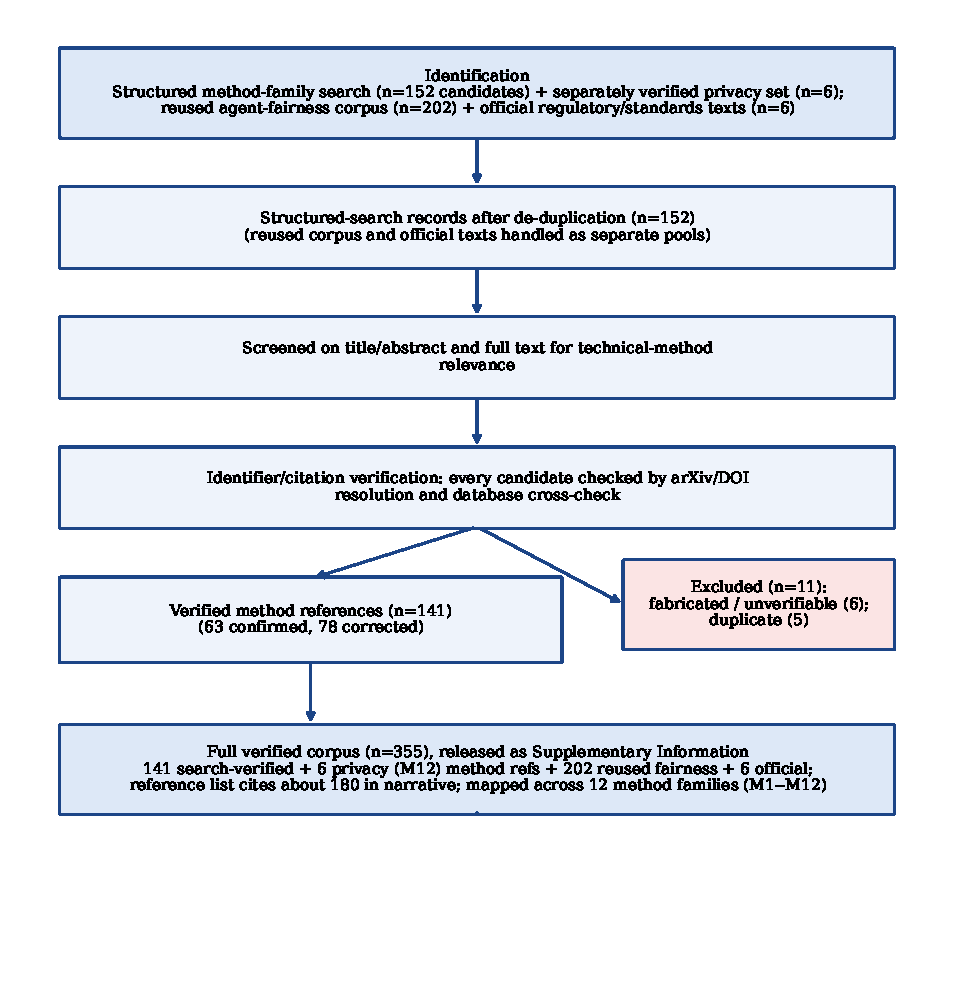
\includegraphics[width=\columnwidth]{../figures/fig_prisma.pdf}
\caption{Record flow of the structured review across the four corpus pools; the
identifier/citation-verification step is described in Section~\ref{sec:method}, and every
transition is reconciled in the released ledger. \textbf{Takeaway:} the corpus is deliberately
focused (152 candidates $\rightarrow$ 141 verified, 11 excluded; 355 records total) but every
transition is auditable end-to-end.}\label{fig:prisma}\end{figure}
This review follows a structured, transparent protocol for a \emph{methods-to-requirements}
mapping. We frame it as a \emph{structured narrative (scoping) review} with a documented,
reproducible search rather than a PRISMA systematic review: the central artifact is an
interpretive crosswalk we make auditable, not a meta-analysis or exhaustive field
enumeration. The protocol was fixed before corpus collection; the search, corpus, coding
ledger, and matrix are released so the synthesis is inspectable.

\subsection{Review Questions}
\textbf{RQ1.} What technical AI evaluation and assessment methods exist, organized by what
they measure? \textbf{RQ2.} Which technical evaluation method could \emph{support an
evidentiary case for conformity} with which requirement of (a)~the NIST AI RMF~1.0,
(b)~the EU AI Act high-risk obligations (Articles~9--15), and (c)~ISO/IEC~42001:2023, and
with what strength of \emph{technical relevance}? \textbf{RQ3.} Which requirements are
weakly served or unserved by technical evaluation methods---i.e., where is the
\emph{measurement gap}?

\subsection{Scope}
We include high-risk and high-stakes AI/ML systems, including large language models (LLMs)
and agentic systems; technical evaluation methods that yield artifacts relevant to
conformity; and the three named frameworks with their official companions. We exclude pure
legal or policy commentary lacking a technical method, consumer/low-risk systems, and
sector regulation outside the three frameworks (cited only for context).

\subsection{Information Sources and Search}
We searched IEEE~Xplore, the ACM Digital Library, Scopus, Web~of~Science, and arXiv
(cs.LG, cs.AI, cs.CY, cs.CR, stat.ML), with forward/backward snowballing via
Google~Scholar. Regulatory requirements were taken from the official corpus: the
NIST~AI~RMF~1.0 (NIST~AI~100-1)~\cite{nist2023airmf} and its Generative~AI
Profile~\cite{nist2024genai}; Regulation~(EU)~2024/1689~\cite{euaiact2024}; and
ISO/IEC~42001:2023~\cite{iso42001} with companion standards. The Boolean search template
combined system terms (AI, machine learning, LLM, foundation model, AI agent) with
evaluation terms (evaluation, assessment, audit, benchmark, testing, assurance, conformity
assessment) and method terms (fairness, robustness, safety, red-teaming, interpretability,
calibration, data governance, model card, human oversight, monitoring), plus a dedicated
governance string. The search window was 2015--2026 with an LLM/agentic emphasis on
2022--2026; the language was English; the last search was conducted in June~2026.
Table~\ref{tab:search} lists the concept groups, and the per-database Boolean query
strings---with the term groups defined and substituted for each database---and the search
dates are released for reproducibility in the companion artifact.

\subsection{The Review Corpus and Its Reconciliation}
To keep the corpus auditable we distinguish four record pools. (i)~A \emph{structured
search} across the twelve families returned candidate technical-method records; after
title/abstract and full-text screening and an identifier/citation-verification step
(below), this yielded \textbf{141} verified technical-method references across families
M1, M3--M11, and governance/positioning; privacy-evaluation methods (M12) were verified
separately as a set of \textbf{6} references, so the released method index contains
\textbf{147} records in total. (ii)~For the
fairness family (M2) we \emph{reuse} a previously published, independently verified
\textbf{202}-entry agent-fairness corpus released separately by the authors; because this
is larger than the bespoke per-family searches, we treat it as a reused supplement and
report a sensitivity analysis with and without it. (iii)~\textbf{Six} official
regulatory/standards texts (the NIST, EU, and ISO anchors and companions) were
hand-collected. (iv)~Two unpublished author manuscripts are mentioned in-text only as
non-independent context and are not listed in the reference list. The complete verified corpus ($\approx$355 records: 147 method $+$ 202 reused $+$ 6
official) is released as Supplementary
Information and in the companion repository, each record carrying metadata, source status,
and family assignment, so that every included record is inspectable. The article's
\emph{reference list} cites approximately \textbf{180} records discussed in the narrative; the
remaining reused-corpus entries are released in full rather than enumerated inline.
Figure~\ref{fig:prisma} shows the record flow, every transition of which is reconciled in
the released ledger.

\emph{Family-level source counts} (newly verified method references) are M1~16, M3~14,
M4~10, M5~13, M6~11, M7~15, M8~12, M9~14, M10~14, M11~12, governance/positioning~10, and
privacy (M12)~6; the fairness family (M2) draws on the reused 202-entry corpus. \emph{Sensitivity:} because the matrix codes
\emph{relevance type} rather than counts, removing the reused fairness corpus changes no
matrix cell and no coverage-breadth rating; its only effect is the relative prominence of
action-level fairness in the research agenda (Section~\ref{sec:gaps}), which we flag.

\subsection{Selection Criteria}
A record was \emph{included} if it (i)~proposed, surveyed, or empirically evaluated a
technical AI evaluation method, or was an official regulatory/standards text;
(ii)~addressed at least one of the twelve method families or framework requirements;
(iii)~had retrievable full text; and (iv)~was in English. A record was \emph{excluded} if
it was opinion/marketing without a method, purely legal analysis without technical
evaluation content, a duplicate, not retrievable, or off-scope (Table~\ref{tab:incl}).

\subsection{Data Extraction}
For each included item we extracted a structured record: bibliographic metadata (authors,
year, venue, DOI/arXiv identifier), a one-line statement of the method contributed, the
assigned method family ($M1$--$M12$), the candidate mapped requirement(s) per framework,
and a technical-relevance code.

\subsection{Coding Protocol and Reliability}
Mapping proceeded in three passes. (1)~\emph{Family assignment}: each method is assigned a
primary family and optional secondary families. (2)~\emph{Requirement mapping}: for every
(method, requirement) pair we assign a technical-relevance level grounded in the official
clause text. \emph{Primary} (\direct): the method produces an artifact that the requirement
chiefly asks for---e.g., an adversarial-robustness report for the EU AI Act Article~15
robustness facet. \emph{Supporting} (\partialev): the artifact feeds a required outcome or
document but is insufficient alone---e.g., a benchmark result is an input to the Article~9
risk-management system but does not constitute it. \emph{Contextual} (\indirect): the
artifact informs the requirement without serving as its evidence---e.g., interpretability
analysis informs governance documentation. A blank denotes non-applicability. The
supporting-versus-blank boundary for process obligations is decided by whether the method's
output is a named input to the obligation's process (supporting) or not (blank).
(3)~\emph{Structured re-examination}: a second pass challenged every non-blank cell against
the clause text and downgraded over-claims (e.g., performance$\rightarrow$Article~11,
safety$\rightarrow$Article~9, the technical$\rightarrow$GOVERN cells, and the privacy
recoding); the full cell-level change log is released.

\emph{Reliability.} A second author independently coded a stratified sample of 40 of the
199 non-blank cells ($\approx$20\%), blind to the first-pass codes. Raw exact agreement was
52.5\% (Cohen's $\kappa=0.18$). We report the unweighted $\kappa$ transparently but note it
is deflated here by two well-understood effects: the marginal distribution is heavily skewed
toward \emph{supporting} (the ``$\kappa$ paradox'', under which high agreement on an
unbalanced category still yields a low $\kappa$), and the scale is a fine three-level ordinal
one on which exact-match $\kappa$ penalizes adjacent codes as harshly as opposite ones. Because
the codes are ordinal, the chance-corrected quadratically-weighted $\kappa$ is the appropriate
measure: all 19 disagreements were a single adjacency level apart, with \emph{no}
primary$\leftrightarrow$contextual conflicts, yielding a quadratically-weighted
$\kappa=0.44$ (moderate). The scheme therefore separates strong from
weak relevance reliably, while the supporting-versus-adjacent boundary is interpretive.
Disagreements were adjudicated to a consensus code; the second
coder's systematically more conservative treatment of governance cells was adopted across
the GOVERN column.

\emph{External validation.} To obtain a check independent of the author team, an external
reviewer (not an author of this study; acknowledged below), blind to the first-pass codes,
recoded the same 40-cell sample. Agreement with the first-pass codes was 57.5\% exact, with
Cohen's $\kappa=0.23$ and a quadratically-weighted $\kappa=0.49$ (computed on the same
relevance scale, here including a single not-applicable code); as in the in-team check, all
17 disagreements were a single adjacency level apart, with \emph{no}
primary$\leftrightarrow$contextual conflicts. The independent recoding
reproduces the same pattern---modest exact agreement on the fine ordinal scale, reliable
separation of strong from weak relevance---which supports presenting the crosswalk as a
\emph{proposed}, externally-checked artifact; broader multi-expert validation would
strengthen it further (Section~\ref{sec:limits}). Both the second-coder and external-validator
cell-level ledgers (\texttt{coding\_audit.csv}, \texttt{external\_validation.csv}) are
released as Supplementary Information.

\subsection{Coverage Breadth}
Per requirement we derive a \emph{coverage-breadth} indicator strictly from the number of
method families with \emph{primary} relevance: \emph{broad} ($\geq$3 families),
\emph{moderate} (1--2), and \emph{narrow} (0). We emphasize that this measures breadth of
mapped families, \emph{not} the methodological maturity, validation quality, or deployment
evidence of the underlying methods; it feeds the gap analysis (Section~\ref{sec:gaps}).

\subsection{Standards Access and Citation Integrity}
Every regulatory obligation is cited to its official source with the specific article,
subcategory, or control identifier. For ISO/IEC~42001:2023 we mapped to the published
Annex~A control structure (numbers and titles) and corroborating secondary analyses of the
standard; protected text is not reproduced beyond permissible quotation. No reference
entered the bibliography without a verified DOI, arXiv identifier, or official document URL
confirmed to resolve; reused entries inherited prior verification and were spot-checked.

\subsection{Threats to Validity}
The crosswalk is interpretive: the frameworks are outcome- and process-oriented and do not
prescribe specific methods, so our cells are reasoned engineering interpretations of
technical relevance, not legal compliance determinations, and a different coder could
assign some adjacent codes differently (the reliability analysis quantifies this). The
frameworks also evolve: EU AI Act application dates were revised by a May~2026 political
agreement, delegated acts and harmonised standards remain in progress, and ISO/IEC
companion standards are emerging (Section~\ref{sec:background}); this review therefore
reflects the state of affairs as of June~2026. Database coverage, English-only inclusion,
preprint inclusion, and the reused fairness corpus introduce selection effects, partly
addressed by the sensitivity analysis above. This article is a technical review and does
\emph{not} constitute legal advice.


\section{A Taxonomy of Technical AI Evaluation Methods}\label{sec:taxonomy}
Building an auditable mapping requires first a principled organization of the evaluation literature. We group technical AI evaluation methods into twelve families by \emph{what they measure}. Table~\ref{tab:taxonomy} summarizes the families; the subsections below describe each, its representative methods, its state of the art for LLM and agentic systems, and its maturity. The families form the rows of the mapping matrix in Section~\ref{sec:mapping}.

% T3 — taxonomy summary
\begin{table*}[!tp]
\centering
\caption{Taxonomy of technical AI evaluation method families. Maturity is assessed for the
LLM/agentic setting; classical-ML maturity is higher in several families. \textbf{Takeaway:}
most families are mature for classical/static models but only \emph{emerging} for LLM and
agentic systems---the maturity frontier, not the method inventory, is where conformity evidence
is currently thin.}
\label{tab:taxonomy}
\footnotesize
\begin{tabular}{p{0.04\textwidth}p{0.17\textwidth}p{0.40\textwidth}p{0.20\textwidth}}
\toprule
ID & Family & Representative methods / metrics & Maturity (LLM/agentic)\\
\midrule
M1 & Performance \& benchmarking & Held-out/OOD test sets, AUROC/F1, significance testing; MMLU, SuperGLUE, BIG-bench, agentic task suites & Mature (classical); evolving (agentic)\\
M2 & Fairness \& bias & Group/individual/counterfactual fairness, disparate impact; BBQ, StereoSet; action-level disparity & Mature (model); emerging (agentic)\\
M3 & Robustness \& distribution shift & PGD/C\&W attacks, randomized smoothing, ImageNet-C, WILDS, prompt-robustness & Mature (vision); emerging (LLM)\\
M4 & Safety evaluation & Hazard analysis, dangerous-capability evals, content-harm benchmarks, safety cases & Emerging\\
M5 & Red-teaming \& adversarial & Structured/automated red-teaming, jailbreaks, (indirect) prompt injection, agent tool-misuse & Emerging, fast-moving\\
M6 & Interpretability \& explainability & Feature attribution (SHAP, LIME, integrated gradients), concept testing (TCAV), probing, mechanistic interp., explanation-faithfulness, CoT faithfulness & Maturing; faithfulness contested\\
M7 & Uncertainty \& calibration & ECE/Brier, conformal prediction, selective prediction, semantic entropy, hallucination detection & Mature (calibration); emerging (LLM)\\
M8 & Data quality, governance \& docs & Datasheets, data cards, provenance audits, contamination/leakage detection, representativeness & Maturing\\
M9 & Transparency \& model documentation & Model/system cards, FactSheets, transparency indices, reproducibility checklists & Maturing\\
M10 & Human oversight \& interaction & Oversight-effectiveness, automation-bias and appropriate-reliance studies, escalation/deferral & Emerging\\
M11 & Post-deployment monitoring \& assurance & Drift detection, runtime monitoring, logging, incident reporting, third-party audit & Emerging\\
M12 & Privacy evaluation & Membership-inference and extraction attacks, differential-privacy verification, model-inversion resistance, privacy-risk assessment & Mature (attacks); emerging (LLM/agentic)\\
\bottomrule
\end{tabular}
\end{table*}




\subsection{M1: Performance \& benchmarking evaluation}

\paragraph{What it measures and why it matters.} The performance and benchmarking family quantifies how accurately and reliably a system maps inputs to correct outputs on held-out and out-of-distribution (OOD) data. This is the most basic conformity claim a deployer can make: that the system performs as intended on representative data and degrades gracefully under shift. Standardized metrics with appropriate statistical treatment are the operational counterpart to the accuracy and documentation expectations of the NIST AI RMF \cite{nist2023airmf}, the EU AI Act \cite{euaiact2024}, and ISO/IEC 42001 \cite{iso42001}.

\paragraph{Representative methods, metrics, and tools.} Classical supervised evaluation reports threshold-based and ranking metrics (accuracy, precision/recall, F1, AUROC) with significance testing on held-out splits, and increasingly assesses OOD generalization and adversarial robustness under shift \cite{li2024oodobustbench}. Calibration is examined alongside raw accuracy to ensure reported confidences are trustworthy \cite{le2024revisiting}. Provenance and reproducibility are documented through model cards \cite{mitchell2019modelcards} and datasheets \cite{gebru2018datasheets}, which record evaluation conditions and intended use. For language systems, aggregate competence is measured on multi-task suites such as MMLU \cite{hendrycks2020mmlu}, SuperGLUE \cite{wang2019superglue}, and the broad BIG-bench collection \cite{srivastava2023bigbench}.

\paragraph{LLM and agentic state of the art.} Contemporary practice extends benchmarking to generative and agentic behavior: instruction-following is scored with debiased automatic evaluators \cite{dubois2024alpacaeval}, factuality with hard multi-turn hallucination benchmarks \cite{hendrycks2024haulaeval}, and prompt-level robustness with adversarial perturbation suites \cite{dong2023promptrobust}. Agentic systems are assessed on end-to-end task completion across architectures \cite{anil2024agentarch}, multi-dimensional enterprise criteria \cite{song2025multidimensional}, and multilingual performance-and-security settings \cite{wang2023maps}. Structured high-stakes evaluation protocols (including a recent unpublished framework; citation withheld for double-blind review) organize these heterogeneous benchmarks into auditable evidence.

\paragraph{Maturity.} Classical ML benchmarking is mature, whereas LLM and agentic benchmarking remains rapidly evolving and contested, with active debate over contamination and construct validity. As summarized in Table~\ref{tab:matrix}, this family principally supplies evidence for accuracy, robustness, and performance-monitoring requirements across all three regimes.

\subsection{M2: Fairness \& bias evaluation}

This family measures whether a system's outputs, predictions, or actions systematically advantage or disadvantage groups defined by protected attributes. Anti-discrimination is an explicit demand across all three regimes: fairness and harmful-bias management is a core NIST trustworthiness characteristic \cite{nist2023airmf}, the EU AI Act requires examination for discriminatory outcomes and appropriate data governance \cite{euaiact2024}, and ISO/IEC 42001 obliges organizations to treat fairness-related impacts within the management system \cite{iso42001}.

\paragraph{Representative methods and metrics.} Classical evaluation distinguishes group fairness, individual fairness, and causal notions, surveyed comprehensively by \textit{Mehrabi et al.} \cite{mehrabi2021survey}. Group criteria include equalized odds and equality of opportunity \cite{hardt2016equality}, while individual fairness formalizes the principle that similar individuals receive similar treatment \cite{dwork2012fairness}. Counterfactual fairness instead conditions on causal interventions over protected attributes \cite{kusner2017counterfactual}. A well-known result is that several group criteria are mutually incompatible except in degenerate cases \cite{kleinberg2017inherent,chouldechova2017fair}, so conformity evidence must state which definition is being satisfied. Foundational audits such as \textit{Gender Shades} \cite{buolamwini2018gender} and embedding-bias analyses \cite{caliskan2017semantics,bolukbasi2016man} established disparate-impact measurement in practice.

\paragraph{LLM and agentic state of the art.} For language models, fairness evaluation has shifted toward benchmark suites: BBQ \cite{parrish2022bbq}, StereoSet \cite{nadeem2021stereoset}, CrowS-Pairs \cite{nangia2020crows}, and BOLD \cite{dhamala2021bold}, consolidated in recent surveys \cite{gallegos2024bias,chu2024fairness,navigli2023biases} and compositional or trust-oriented batteries \cite{wang2024ceb,huang2024trustllm,wang2023decodingtrust}, alongside dialect-level disparities in reward models \cite{mire2025rejected}. The agentic frontier moves from text to decisions: action-level disparity \cite{li2025actions}, tool-selection bias \cite{blankenstein2025biasbusters}, multi-agent fairness frameworks \cite{ranjan2025fairness}, and a recent agent-fairness framework (citation withheld for double-blind review), which attributes per-component fairness across an agent pipeline.

\paragraph{Maturity.} Static-classifier fairness is mature with established metrics, whereas LLM and agent action-level fairness remain emerging and benchmark-sensitive. This evidence speaks primarily to the discrimination and fairness obligations mapped in Table~\ref{tab:matrix} across NIST, the EU AI Act, and ISO/IEC 42001.

\subsection{M3: Robustness \& distribution-shift evaluation}

This family measures whether a model's predictive quality and safety properties persist when inputs deviate from the training distribution, whether through naturally occurring shift, accidental corruption, or adversarial manipulation. Because high-risk systems are rarely deployed in conditions identical to those under which they were trained, robustness evidence directly substantiates claims about reliability and resilience under foreseeable misuse and operating conditions \cite{nist2023airmf,euaiact2024}.

\paragraph{Representative methods and metrics.} Adversarial robustness has a mature evaluative core: gradient-based attacks such as PGD provide a standard adversarial-accuracy stress test \cite{madry2018pgd,goodfellow2015explaining}, and stronger optimization-based attacks expose models whose apparent robustness is an artifact of weak attacks \cite{carlini2016c2}. Certified methods complement empirical attacks by yielding provable radii within which predictions cannot change, most prominently randomized smoothing \cite{cohen2019certified}. Corruption robustness is quantified against systematic perturbation suites \cite{hendrycks2019corruption} and naturally occurring hard cases \cite{hendrycks2019natural}, while distribution-shift generalization is assessed on curated in-the-wild benchmarks \cite{koh2021wilds} and through methods that target invariance across environments \cite{arjovsky2019irm}. Out-of-distribution detection \cite{liang2024ood} and test-time adaptation, evaluated under realistic unsupervised hyperparameter selection \cite{tta2024realistic}, address whether a system can flag or absorb inputs it should not confidently process.

\paragraph{LLM and agentic state of the art.} For language models, robustness evaluation has shifted toward prompt sensitivity and jailbreak resistance. Standardized jailbreak benchmarks \cite{jailbreakbench2024} and randomized-perturbation defenses \cite{smoothllm2023} measure resilience to adversarial prompting, prompt-sensitivity probes quantify brittleness under benign paraphrase \cite{brittlebench2025}, and data-poisoning benchmarks assess training-time vulnerability \cite{poisonbench2024}; the generative-AI profile frames these as managed risks \cite{nist2024genai}.

\paragraph{Maturity.} Vision robustness and certified methods are mature, whereas LLM and agentic prompt-robustness evaluation remains emerging. As mapped in Table~\ref{tab:matrix}, this evidence speaks most directly to accuracy, robustness, and cybersecurity obligations \cite{euaiact2024}, the NIST resilience and risk-management functions \cite{nist2023airmf}, and operational controls \cite{iso42001}.

\subsection{M4: Safety evaluation}

\paragraph{What it measures and why it matters} The safety family quantifies a system's propensity to cause or enable harm, spanning hazard identification, dangerous-capability elicitation, content-harm measurement, and the structured argumentation that ties such evidence to an acceptable-risk conclusion. It underpins the risk-management and harm-mitigation obligations of all three regimes \cite{nist2023airmf,euaiact2024,iso42001}, and for frontier models is the principal artifact showing that residual hazards have been characterized rather than merely asserted.

\paragraph{Representative methods, metrics, and tools} Content-harm benchmarks operationalize safety as measurable rates of unsafe responses: \textit{SafetyBench} structures multiple-choice probes across harm categories \cite{wang2023safetybench}, while \textit{TruthfulQA} targets the related failure of confidently reproducing human falsehoods \cite{lin2021truthfulqa}. Mitigation-oriented training such as Safe RLHF separates helpfulness from harmlessness so that safety can be tuned and audited as an explicit objective \cite{dai2024saferlhf}. At the assurance level, structured safety cases assemble claims, arguments, and evidence into an auditable conformity narrative \cite{hawkins2025safetycaseai}, and risk-perspective analyses examine whether layered alignment mechanisms constitute independent defenses or share common failure modes \cite{gal2025alignment}.

\paragraph{LLM and agentic state of the art} Frontier evaluation has shifted toward eliciting \textit{dangerous capabilities} (for example cyber-offense, deception, and self-proliferation) under adversarial conditions to bound worst-case misuse potential \cite{hendel2024dangerouseval}. Because such measurements are sensitive to attack strategy, jailbreak-evaluation toolkits standardize how successful circumvention is judged and aggregated \cite{akhtar2024jailbreakeval}, and the NIST Generative AI Profile catalogs the corresponding risk categories and suggested actions \cite{nist2024genai}. For agentic systems, capability elicitation increasingly targets multi-step tool-use trajectories rather than single completions.

\paragraph{Maturity} Content-harm benchmarking and red-team-style jailbreak evaluation are comparatively mature, whereas dangerous-capability elicitation and quantified safety cases remain emerging and contested. As mapped in Table~\ref{tab:matrix}, this evidence speaks most directly to risk-identification, harm-mitigation, and accuracy--robustness obligations across the three frameworks \cite{nist2023airmf,euaiact2024,iso42001}.

\subsection{M5: Red-teaming \& adversarial testing}

This family measures whether a system can be induced to violate its intended safety policy under adversarial pressure, rather than under benign use. It probes for failure modes that ordinary functional testing does not surface: jailbreaks that bypass alignment guardrails, prompt injection (including \textit{indirect} injection routed through retrieved or tool-returned content), and tool-misuse by autonomous agents. Regulators frame robustness and security against adversarial manipulation as an obligation distinct from accuracy, to be assessed before and during deployment \cite{euaiact2024,nist2023airmf}.

\paragraph{Representative methods, metrics, and tools.} Optimization-based attacks generate transferable adversarial suffixes that defeat aligned models \cite{zou2023universal}, while query-efficient black-box methods elicit harmful completions in few interactions \cite{carlini2023extracting}. Standardized harnesses make these results comparable: HarmBench formalizes automated red-teaming and robust-refusal scoring across attack and defense pairs \cite{mazeika2024harmbench}, and benchmark suites quantify instruction-following robustness to prompt injection \cite{hendrycks2023advbench}. Indirect injection has been characterized both as a real-world compromise vector for LLM-integrated applications \cite{greshake2023notwhat} and through dedicated benchmarks that test whether firewalls or stronger evaluations are needed \cite{wang2024indirect}, with prompt-tuning shields proposed as lightweight countermeasures \cite{rai2024soft}. Typical metrics are attack success rate, refusal rate, and transferability across models and prompts.

\paragraph{LLM and agentic state of the art.} Red-teaming is increasingly automated and learning-based, with adversarial generators trained to discover robustness failures at scale \cite{kang2025learning,liu2025automatic}. Agentic evaluation extends the threat surface to tool calls and actions: Agent-SafetyBench measures unsafe agent behavior \cite{zhang2024agent}, SafeSearch red-teams search agents \cite{gu2025safesearch}, and EU-Agent-Bench scores illegal agent actions against legal baselines \cite{peng2025eu}. Recent systematization consolidates these methodologies for assurance and security \cite{wang2026systematic}.

\paragraph{Maturity.} Attack methods and benchmarks are mature for single-turn LLMs but emerging for indirect-injection and agentic tool-misuse settings, where standardization is incomplete. As mapped in Table~\ref{tab:matrix}, it evidences robustness and adversarial-security requirements across the three frameworks and their operational controls \cite{nist2024genai,iso42001}.

\subsection{M6: Interpretability \& explainability evaluation}

This family measures the extent to which a model's internal computations and outputs can be explained, attributed to inputs, and verified as faithful to the model's actual decision process. Such evidence underpins transparency, human oversight, and the ability to interrogate a decision; it speaks to the explainability and transparency expectations of the NIST AI RMF \cite{nist2023airmf}, the documentation and human-oversight obligations of the EU AI Act \cite{euaiact2024}, and the operational-control evidence required by ISO/IEC 42001 \cite{iso42001}.

\paragraph{Representative methods and metrics.} Feature-attribution techniques such as integrated gradients provide axiomatically grounded importance scores \cite{sudre2024axiomatic_integrated_gradients}, while concept-based approaches like Testing with Concept Activation Vectors (TCAV) quantify a model's sensitivity to human-interpretable concepts beyond raw features \cite{kim2019tcav}. Probing classifiers assess what linguistic and structural information is encoded in contextual representations \cite{tenney2019edge_probing}, building on the transformer architecture that motivates much of this analysis \cite{vaswani2017transformer}. A recurrent concern is whether such explanations are faithful rather than merely plausible: attention weights, for instance, have been shown not to constitute reliable explanations \cite{jain2019attention_not_explanation}. Benchmarking efforts such as XAI-Units introduce unit-test-style evaluation to verify that explainability methods behave as specified \cite{yang2024xai_units}.

\paragraph{LLM and agentic state of the art.} For generative and reasoning models, evaluation has shifted toward the faithfulness of chain-of-thought (CoT) traces \cite{yang2023measuring_faithfulness_cot}, with work distinguishing faithfulness from surface plausibility \cite{turpin2024faithfulness_plausibility} and arguing that self-explanations can still help predict model behavior \cite{lanham2024positive_case_faithfulness}. Mechanistic interpretability increasingly probes the internal circuitry of CoT via sparse autoencoding \cite{zou2024cot_mechanistic} and applies causal tracing to localize object representations and mitigate hallucination in vision-language models \cite{zhang2024causal_tracing_vqa}.

\paragraph{Maturity.} Attribution and probing are relatively \textit{mature}, whereas CoT-faithfulness and mechanistic interpretability remain \textit{emerging}. As mapped in Table~\ref{tab:matrix}, this family supplies evidence for transparency, explainability, and human-oversight requirements across all three regimes \cite{nist2023airmf,euaiact2024,iso42001}.

\subsection{M7: Uncertainty quantification \& calibration}

This family measures whether a model's stated confidence corresponds to its empirical correctness, and whether it can abstain or flag low-confidence outputs rather than asserting them. Regulators expect high-risk systems to expose the limits of their reliability: NIST frames calibrated uncertainty under the \textit{Measure} function as a precondition for validly characterized systems \cite{nist2023airmf}, the EU AI Act ties accuracy and robustness disclosures to technical documentation and instructions of use \cite{euaiact2024}, and ISO/IEC 42001 anchors them in performance evaluation and monitoring \cite{iso42001}.

\paragraph{Representative methods and metrics.} Classical calibration is assessed through expected calibration error (ECE) and Brier-type scores, with temperature scaling established as a strong post-hoc remedy for the overconfidence of modern networks \cite{guo2017calibration}, and broader surveys cataloguing the state of the art \cite{wang2023calibration}. Predictive uncertainty itself is estimated via Bayesian approximations such as Monte Carlo dropout \cite{gal2016bayesian}, evidential formulations for classification \cite{sensoy2018evidential} and regression \cite{amini2020deepevidential}, and learned confidence for out-of-distribution detection \cite{devries2018confidence}. Conformal prediction supplies distribution-free coverage guarantees and abstention-ready prediction sets \cite{angelopoulos2023conformal}, with work disentangling its interaction with deep model uncertainty \cite{barella2023quantifying} and isolating epistemic components \cite{ravi2026epistemic}; such sets have been shown to improve human decision making \cite{cresswell2024conformal}.

\paragraph{LLM and agentic state of the art.} For generative models, semantic uncertainty marginalizes over meaning-equivalent generations \cite{kuhn2023semantic}, with cheaper semantic-entropy probes \cite{kossen2024semantic} and token-level temperature scaling refining the estimate \cite{lamb2026temperature}. Zero-resource consistency checks detect hallucination without ground truth \cite{manakul2023selfcheckgpt}, while selective prediction reduces unnecessary abstention in multimodal reasoning \cite{srinivasan2024selective}; the GenAI Profile elevates confabulation and factuality as named risks \cite{nist2024genai}.

\paragraph{Maturity.} Tabular and vision calibration and conformal methods are mature, whereas LLM-level semantic uncertainty and hallucination detection remain emerging and contested. As mapped in Table~\ref{tab:matrix}, this evidence speaks chiefly to accuracy, robustness, and reliability-disclosure obligations across all three frameworks.

\subsection{M8: Data quality, governance \& documentation}
\label{subsec:m8}

This family assesses the data on which high-risk AI systems are built and the artifacts that record how that data was collected, curated, and used. Rather than probing model behavior directly, it measures upstream properties: quality dimensions such as completeness, accuracy, and consistency; representativeness relative to the deployment population; provenance and licensing of training corpora; and the existence and quality of documentation. Regulators treat data governance as a precondition for trustworthy outputs: the EU AI Act requires training, validation, and testing datasets to be relevant, sufficiently representative, and examined for bias \cite{euaiact2024}; the NIST AI RMF locates these concerns in its \textit{Map} and \textit{Measure} functions \cite{nist2023airmf}; and ISO/IEC 42001 requires documented controls over data resources and their lifecycle \cite{iso42001}.

\paragraph{Representative methods and tools.} Structured documentation artifacts are the most established evidence type, spanning Data Cards \cite{pushkarna2022datacards}, model and audit cards \cite{liang2024whatsdocumented,staufer2025auditcards}, and broader transparency instruments \cite{raffel2024transparency,winecoff2024governance}. Data-quality assessment is supported by surveys of quality dimensions and tooling \cite{pan2024metrics}, representativeness and downstream-fairness analyses \cite{liang2024representativeness}, and large-scale provenance and licensing audits \cite{luccioni2023dataprovenance}; provenance can also be captured automatically at the framework level \cite{pocock2021tribuo}. Benchmark and dataset catalogues further inform what evaluation data is available and appropriate \cite{ivanov2024benchmarks}.

\paragraph{LLM and agentic state of the art.} For large language models, the dominant emerging concern is data contamination, where benchmark items leak into pretraining corpora and inflate measured performance; detection methods and their limits are now actively surveyed \cite{lukoševičius2024contamination}. The opacity of web-scale corpora also makes provenance, licensing, and representativeness substantially harder to establish than in the curated-dataset setting \cite{luccioni2023dataprovenance,nist2024genai}.

\paragraph{Maturity.} Documentation templates and quality-dimension tooling are mature, whereas contamination detection, automated provenance tracking, and quantitative representativeness auditing remain emerging \cite{global2024governance}. As mapped in Table~\ref{tab:matrix}, it speaks most directly to data-governance, dataset-representativeness, record-keeping, and transparency requirements.

\subsection{M9: Transparency \& model documentation}
\label{subsec:m9}

This family measures whether an AI system's design, training data, intended use, evaluation results, and known limitations are recorded in a structured, verifiable, and externally legible form. Unlike performance families that score model behavior, M9 assesses the quality and completeness of the \textit{evidentiary record} itself: documentation is the connective tissue that lets an auditor trace a claim back to the test that supports it. This makes the family foundational for conformity, because most regulatory regimes treat the absence of adequate documentation as a deficiency in its own right, independent of how the underlying system performs.

Representative methods center on standardized artifacts and the pipelines that produce and grade them. AI FactSheets propose a supplier-side methodology for declaring system facts across the lifecycle \cite{weidinger2024aifactsheets}, while EvalCards standardize how evaluation results are reported \cite{lin2025evalcards} and model-reporting proposals explicitly merge EU regulatory fields into developer documentation \cite{pan2024modelreporting}. Scoring instruments operationalize transparency as a measurable quantity: the Foundation Model Transparency Index ranks developers against disclosure indicators \cite{wan2025fmti}, and the AI Transparency Atlas adds a real-time model-card evaluation pipeline \cite{shah2025aitransparencyatlas}. Domain extensions, such as bias-aware clinical model cards \cite{tong2024benchmarking}, and global information-exchange frameworks \cite{weidinger2023framework} broaden the documentation surface, while reproducibility programs supply the experimental-evidence backbone \cite{pineau2020reproducibility}. A recent unpublished framework (citation withheld for double-blind review) contributes a structured documentation-and-reporting schema for high-stakes systems.

For LLMs and agentic systems the state of the art is consolidating: surveys map explainability and transparency techniques for large models \cite{zhang2025transparentai,liang2023aiglmsurvey}, empirical-study guidelines target LLM evidence quality \cite{mehdipour2025evaluation}, benchmark-of-benchmarks audits scrutinize the validity of reported scores \cite{qian2025benchmark2}, and the AI Agent Index documents technical and safety features of deployed agents \cite{li2025aiagentindex}. Case studies confirm that documentation methodologies can be evaluated empirically \cite{yang2024evaluating}.

The family is \textit{mature} for static models and \textit{emerging} for agentic and continuously updated systems. As mapped in Table~\ref{tab:matrix}, it evidences NIST \textsc{Govern}/\textsc{Map} documentation functions \cite{nist2023airmf,nist2024genai}, EU AI Act technical-documentation and transparency obligations \cite{euaiact2024}, and the documented-information and lifecycle controls of ISO/IEC 42001 \cite{iso42001}.

\subsection{M10: Human oversight \& human--AI interaction evaluation}
\label{subsec:m10}

This family measures whether a human retained in the loop can meaningfully understand, supervise, and correct an AI system in operation. Rather than scoring the model in isolation, it evaluates the joint human--AI decision unit along dimensions such as oversight effectiveness, automation bias, appropriate (calibrated) reliance, contestability, and the reliability of escalation or deferral pathways. Regulators treat human oversight as a primary risk control: it is a governance and measurement expectation under the NIST AI RMF \textit{Govern} and \textit{Measure} functions \cite{nist2023airmf}, a binding high-risk obligation under the EU AI Act \cite{euaiact2024}, and an operational control an AI management system must implement and audit under ISO/IEC 42001 \cite{iso42001}.

\paragraph{Representative methods, metrics, and tools.} Trust-calibration surveys frame the target construct as alignment between user trust and actual system reliability \cite{amershi2022trustcalibration}, and decision-theoretic formulations operationalize ``appropriate reliance'' as a measurable quantity rather than raw agreement \cite{guo2024reliance}. Reviews of automation bias catalogue when explanations help or harm oversight \cite{romeo2025automationbias}, motivating human-aligned XAI benchmarks \cite{wang2024xaibenchmark} and studies of how operators form mental models during collaboration \cite{wang2025mentalmodels}. Reliance drills probe over-dependence by injecting controllable errors \cite{chen2024reliancedrills}, while staged evaluation workflows integrate domain experts and lay users into the assessment loop \cite{liang2024stagedworkflows}, and system cards externalize oversight assumptions for review \cite{reddy2025systemcards}.

\paragraph{LLM and agentic state of the art.} For reasoning models, process-level supervision and step-by-step verification expose intermediate steps for human checking \cite{wang2023verifystepbystep,hou2025processrewardsurvey}, and interactive-alignment views treat oversight as continuous specification negotiation \cite{krause2023interactivealignment}. Agentic settings add escalation and deferral evaluation \cite{cui2024escalation}, action-level assessment beyond task completion \cite{tan2024agentassessment}, and constitution-based behavioral constraints \cite{tan2025constitutionalai}.

\paragraph{Maturity.} The family is \textit{emerging}: trust-calibration and automation-bias constructs are well established, but standardized oversight metrics for agentic systems remain immature. This evidence speaks primarily to the human-oversight and transparency requirements mapped in Table~\ref{tab:matrix}.

\subsection{M11: Post-deployment monitoring \& assurance}

This family measures whether a deployed system continues to behave within its validated operating envelope, and whether deviations are detected, logged, and escalated in a timely manner. Since pre-deployment evaluation captures only a snapshot, post-deployment monitoring is the evidentiary backbone of \textit{continuous} conformity: it speaks to the \textsc{Manage}-function operate-and-monitor obligations of the NIST AI RMF \cite{nist2023airmf}, to post-market monitoring, logging, and serious-incident reporting under the EU AI Act \cite{euaiact2024}, and to the performance-evaluation and continual-improvement clauses of ISO/IEC 42001 \cite{iso42001}.

\paragraph{Representative methods, metrics, and tools.} Core techniques include distribution-shift and concept-drift detection over inputs and learned representations \cite{greco2024driftlens,neuralnetwork2024robustness}, contextualized runtime monitoring that maps signals to operating context rather than raw statistics \cite{leest2025contextaware}, and uncertainty quantification used as a live trigger for shift and degradation \cite{neuralnetwork2024robustness}. Lifecycle-oriented frameworks organize these signals into structured assurance and traceable terminology \cite{aisystem2024evaluation}, while scalable policy-checking pipelines automate continuous compliance evaluation against codified requirements \cite{compliance2025pasta}. On the assurance side, third-party and frontier-model auditing methodologies \cite{auditing2024frontier}, layered governance-and-certification architectures \cite{audit2025responsible}, adaptive governance for decentralized deployment \cite{governance2025adaptive}, and incident-analysis taxonomies that convert reported harms into actionable patterns \cite{incidents2025harms} provide the external-evidence layer.

\paragraph{LLM and agentic state of the art.} For generative systems, monitoring increasingly targets factuality: decoding-time hallucination monitors that score partial responses during generation \cite{monitoring2025hallucination} and fact-checking pipelines that score factuality of deployed outputs \cite{mitigating2025hallucination}. For agentic systems, a recent agent-fairness framework (citation withheld for double-blind review) extends runtime monitoring to per-component, action-level disparity, attributing fairness drift to the responsible agent step rather than the aggregate output.

\paragraph{Maturity.} Drift detection and logging are mature; continuous agentic assurance, third-party audit, and live hallucination monitoring remain emerging. As summarized in Table~\ref{tab:matrix}, this evidence maps to the \textsc{Manage}/monitor, post-market monitoring and incident-reporting, and performance-evaluation requirements of the three regimes \cite{nist2023airmf,euaiact2024,iso42001}.

\subsection{M12: Privacy evaluation}

This family measures whether a system leaks information about the individuals in its
training data or the subjects of its inputs, and whether privacy-protective techniques
provide their claimed guarantees. Privacy is one of the trustworthiness characteristics
that high-risk regimes require be assessed: it is named explicitly in the NIST AI RMF
(\textsc{Measure}~2.10)~\cite{nist2023airmf}, underlies the data-governance and
transparency duties of the EU AI Act~\cite{euaiact2024}, and is a core impact dimension of
the ISO/IEC~42001 impact-assessment controls~\cite{iso42001}.

\paragraph{Representative methods and metrics.} The dominant empirical instruments are
attacks repurposed as audits. Membership-inference attacks estimate whether a given record
was in the training set and have become a standard privacy-leakage
metric~\cite{shokri2017membership}, with later work placing their evaluation on rigorous,
likelihood-ratio foundations to avoid overstated robustness~\cite{carlini2022firstprinciples}.
Training-data-extraction attacks demonstrate verbatim memorisation in large language
models, providing a direct, alarming measure of leakage~\cite{carlini2021extracting}, while
inference attacks show that models can expose attributes never explicitly
stated~\cite{staab2023memorization}. On the defensive side, differential privacy supplies a
provable guarantee whose privacy budget is itself the evaluation
metric~\cite{abadi2016dp}.

\paragraph{LLM and agentic state of the art.} Privacy evaluation for LLMs and agents is an
active and consolidating area, surveyed comprehensively in recent
work~\cite{neel2023privacy}; open problems include quantifying leakage through tool use and
retrieval, and evaluating memorisation at frontier scale.

A caveat governs how this family maps to conformity: most of its instruments are
\emph{vulnerability tests} (membership-inference, extraction, attribute-inference) that
\emph{detect} privacy leakage rather than \emph{assure} its absence. They evidence that a
privacy risk was examined, in keeping with the EU AI Act and ISO impact-assessment framing, but do not by
themselves demonstrate privacy adequacy; differential privacy is the exception, supplying a
provable guarantee. We therefore code privacy evaluation as having \emph{supporting} rather
than \emph{primary} relevance to the privacy requirement (NIST \textsc{Measure}~2.10).

\paragraph{Maturity.} Attack-based leakage measurement and differential-privacy accounting
are mature for classical models but unevenly applied to LLMs and agentic pipelines, and
this family is, relative to the others, comparatively thin in our corpus. As shown in
Table~\ref{tab:matrix}, it is the main \emph{partial}-evidence source for the privacy
requirements of all three frameworks; the privacy requirement itself is consequently
flagged as weakly served in the gap analysis (Section~\ref{sec:gaps}).


\section{Mapping Evaluation Methods to Regulatory Requirements}\label{sec:mapping}
\begin{figure*}[!tp]\centering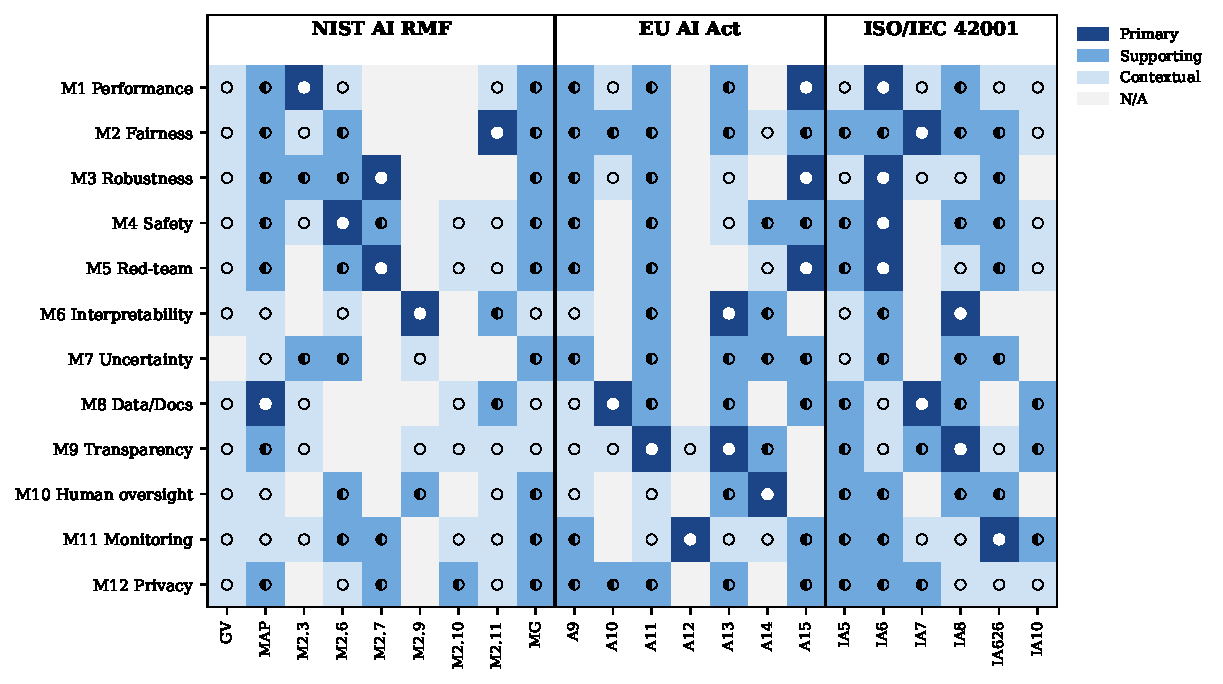
\includegraphics[width=0.92\textwidth]{../figures/fig_heatmap.pdf}
\caption{Heatmap of the proposed crosswalk: technical relevance of each method family (rows)
for each requirement (columns), grouped by framework. \CIRCLE~primary, \LEFTcircle~supporting,
\Circle~contextual technical relevance (filled, half-filled, and empty circle, respectively).
\textbf{Takeaway:} primary-relevance evidence concentrates on the measurable trustworthiness
characteristics (accuracy, robustness, security, explainability, fairness), while the process,
human-oversight, and agentic columns are visibly sparse---previewing the gap analysis.}\label{fig:heatmap}\end{figure*}
\begin{figure*}[!tp]\centering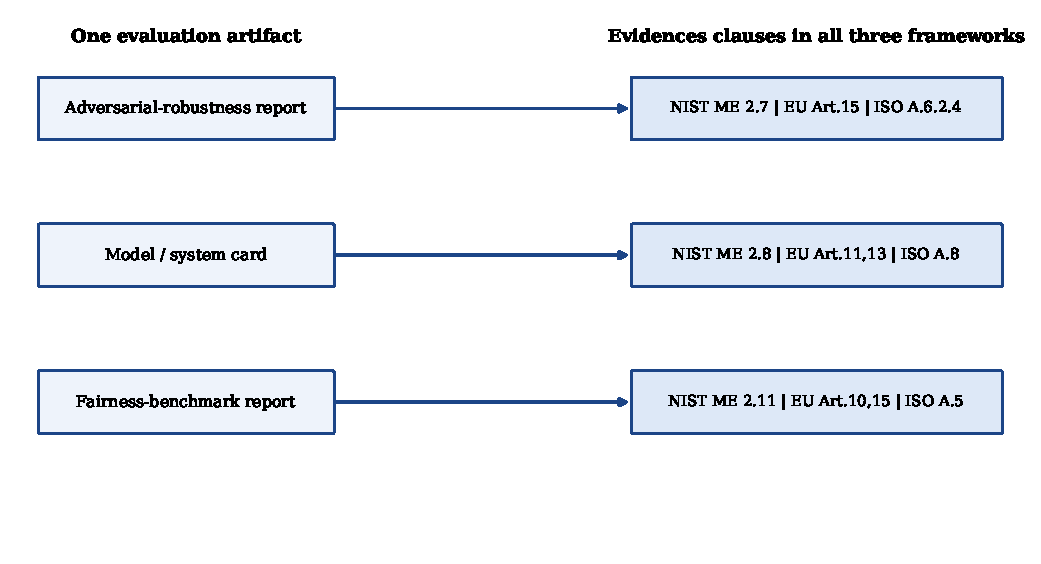
\includegraphics[width=0.82\textwidth]{../figures/fig_crosswalk.pdf}
\caption{Cross-framework crosswalk: a single evaluation artifact is typically relevant to
clauses in all three frameworks simultaneously. \textbf{Takeaway:} because one artifact (e.g.,
an adversarial-robustness report or a model card) evidences NIST, EU, and ISO clauses at once,
the marginal cost of multi-framework conformity is far below running three separate
programs.}\label{fig:crosswalk}\end{figure*}
This section presents the central contribution: a mapping from the twelve technical
evaluation method families of Section~\ref{sec:taxonomy} to the requirements of the three
frameworks. We first state the coding scheme, then walk each framework, and close with a
cross-framework crosswalk. The full mapping is given in Table~\ref{tab:matrix} and
visualized in Fig.~\ref{fig:heatmap}.

\subsection{Technical-relevance coding}
For each (method family, requirement) pair we assign one of three levels of \emph{technical
relevance}, capturing how far the method's output could contribute to an evidentiary case for the
requirement, grounded in the official clause text. We code \emph{relevance}, not legal
sufficiency: a technical artifact rarely demonstrates conformity by itself, its adequacy
depending on intended purpose, applicable harmonised standards, acceptance criteria, and the
conformity-assessment route. \emph{Primary} (\direct): the output is itself the kind of
technical evidence the requirement chiefly asks for. \emph{Supporting} (\partialev): the
method contributes but is insufficient alone. \emph{Contextual} (\indirect): it informs the
requirement without serving as its evidence. A blank denotes non-applicability. Codes were
assigned in a first pass grounded in clause text, then challenged in a structured second
pass, with a second author independently coding a stratified sample (Section~\ref{sec:method}).
The coding is an interpretive engineering judgment (Section~\ref{sec:limits}); we present the
matrix as a \emph{proposed} crosswalk inviting external validation, not an established map of
what demonstrates conformity.

\paragraph{Worked example} To make the coding transparent, consider EU AI Act Article~15,
which requires high-risk systems to achieve ``appropriate levels of accuracy, robustness
and cybersecurity''~\cite{euaiact2024}. Performance and benchmarking (M1) has
\emph{primary} relevance to the accuracy dimension through held-out and out-of-distribution
test results; robustness and distribution-shift evaluation (M3) has \emph{primary} relevance
to robustness through adversarial and corruption tests; red-teaming (M5) has \emph{primary}
relevance to resilience to manipulation; uncertainty and calibration (M7) has only
\emph{supporting} relevance, since it characterizes the reliability of accuracy claims but
not adversarial security; and interpretability (M6) is not applicable to this
clause. Applying this logic clause by clause against the official text produces every cell
of Table~\ref{tab:matrix}.

% Auto-generated signature matrix (Table T4). Glyph macros defined in main.tex.
\begin{sidewaystable*}
\centering
\caption{Proposed methods-to-requirements crosswalk (the article\textquotesingle s central artifact): technical evaluation method families (rows) against regulatory requirements (columns). Each cell records the authors\textquotesingle{} interpretive coding of the method\textquotesingle s \emph{technical relevance} to the requirement: \direct~primary, \partialev~supporting, \indirect~contextual; a blank denotes not applicable. The codes are an engineering judgment grounded in the official clause text, not a legal determination of conformity; a second author independently coded a stratified 20\% sample (Section~\ref{sec:method}). NIST AI RMF functions/subcategories~\cite{nist2023airmf}, EU AI Act high-risk Articles~\cite{euaiact2024}, ISO/IEC 42001 Annex~A controls~\cite{iso42001}. ISO columns: A.5 assessing impacts, A.6.2.4 verification and validation, A.7 data for AI systems, A.8 information for interested parties, A.6.2.6 operation and monitoring, A.10 third-party relationships. Rotate the page 90$^\circ$ to read the column headers; Fig.~\ref{fig:heatmap} provides a visual overview of the same data.}
\label{tab:matrix}
\footnotesize
\setlength{\tabcolsep}{3pt}
\begin{tabular}{lcccccccccccccccccccccc}
\toprule
 & \multicolumn{9}{c}{\textbf{NIST AI RMF}} & \multicolumn{7}{c}{\textbf{EU AI Act}} & \multicolumn{6}{c}{\textbf{ISO/IEC 42001}}\\
\cmidrule(lr){2-10}\cmidrule(lr){11-17}\cmidrule(lr){18-23}
\textbf{Method family} & \rotatebox{90}{NIST GOVERN} & \rotatebox{90}{NIST MAP} & \rotatebox{90}{ME 2.3 Acc.} & \rotatebox{90}{ME 2.6 Safety} & \rotatebox{90}{ME 2.7 Sec.} & \rotatebox{90}{ME 2.9 Expl.} & \rotatebox{90}{ME 2.10 Priv.} & \rotatebox{90}{ME 2.11 Fair} & \rotatebox{90}{NIST MANAGE} & \rotatebox{90}{Art.9} & \rotatebox{90}{Art.10} & \rotatebox{90}{Art.11} & \rotatebox{90}{Art.12} & \rotatebox{90}{Art.13} & \rotatebox{90}{Art.14} & \rotatebox{90}{Art.15} & \rotatebox{90}{A.5 Impact} & \rotatebox{90}{A.6.2.4 V\&V} & \rotatebox{90}{A.7 Data} & \rotatebox{90}{A.8 Info} & \rotatebox{90}{A.6.2.6 Mon.} & \rotatebox{90}{A.10 3rd-pty}\\
\midrule
M1~Performance \& benchmarking & \indirect & \partialev & \direct & \indirect &  &  &  & \indirect & \partialev & \partialev & \indirect & \partialev &  & \partialev &  & \direct & \indirect & \direct & \indirect & \partialev & \indirect & \indirect\\
M2~Fairness \& bias evaluation & \indirect & \partialev & \indirect & \partialev &  &  &  & \direct & \partialev & \partialev & \partialev & \partialev &  & \partialev & \indirect & \partialev & \partialev & \partialev & \direct & \partialev & \partialev & \indirect\\
M3~Robustness \& distribution shift & \indirect & \partialev & \partialev & \partialev & \direct &  &  &  & \partialev & \partialev & \indirect & \partialev &  & \indirect &  & \direct & \indirect & \direct & \indirect & \indirect & \partialev & \\
M4~Safety evaluation & \indirect & \partialev & \indirect & \direct & \partialev &  & \indirect & \indirect & \partialev & \partialev &  & \partialev &  & \indirect & \partialev & \partialev & \partialev & \direct &  & \partialev & \partialev & \indirect\\
M5~Red-teaming \& adversarial testing & \indirect & \partialev &  & \partialev & \direct &  & \indirect & \indirect & \partialev & \partialev &  & \partialev &  &  & \indirect & \direct & \partialev & \direct &  & \indirect & \partialev & \indirect\\
M6~Interpretability \& explainability & \indirect & \indirect &  & \indirect &  & \direct &  & \partialev & \indirect & \indirect &  & \partialev &  & \direct & \partialev &  & \indirect & \partialev &  & \direct &  & \\
M7~Uncertainty \& calibration &  & \indirect & \partialev & \partialev &  & \indirect &  &  & \partialev & \partialev &  & \partialev &  & \partialev & \partialev & \partialev & \indirect & \partialev &  & \partialev & \partialev & \\
M8~Data quality, governance \& docs & \indirect & \direct & \indirect &  &  &  & \indirect & \partialev & \indirect & \indirect & \direct & \partialev &  & \partialev &  & \partialev & \partialev & \indirect & \direct & \partialev &  & \partialev\\
M9~Transparency \& model documentation & \indirect & \partialev & \indirect &  &  & \indirect & \indirect & \indirect & \indirect & \indirect & \indirect & \direct & \indirect & \direct & \partialev &  & \partialev & \indirect & \partialev & \direct & \indirect & \partialev\\
M10~Human oversight \& interaction & \indirect & \indirect &  & \partialev &  & \partialev &  & \indirect & \partialev & \indirect &  & \indirect &  & \partialev & \direct &  & \partialev & \partialev &  & \partialev & \partialev & \\
M11~Post-deployment monitoring \& assurance & \indirect & \indirect & \indirect & \partialev & \partialev &  & \indirect & \indirect & \partialev & \partialev &  & \indirect & \direct & \indirect & \indirect & \partialev & \partialev & \partialev & \indirect & \indirect & \direct & \partialev\\
M12~Privacy evaluation & \indirect & \partialev &  & \indirect & \partialev &  & \partialev & \indirect & \partialev & \partialev & \partialev & \partialev &  & \partialev &  & \partialev & \partialev & \partialev & \partialev & \indirect & \indirect & \indirect\\
\bottomrule
\end{tabular}
\end{sidewaystable*}


\subsection{Mapping to the NIST AI RMF}\label{sec:map-nist}
The NIST AI RMF concentrates technical measurement in the \textsc{Measure} function,
whose subcategories enumerate the trustworthiness characteristics to be
evaluated~\cite{nist2023airmf}. Throughout, we use NIST's official \textsc{Measure}~2.x
subcategory numbering (notably 2.3 performance, 2.5 validity and reliability, 2.6 safety,
2.7 security and resilience, 2.8 transparency and accountability, 2.9 explainability and
interpretability, 2.10 privacy, and 2.11 fairness and harmful bias managed). The matrix columns cover the
trustworthiness-characteristic subcategories most directly tied to technical evaluation;
the remaining subcategories (\textsc{Measure}~2.1, test
documentation; 2.2, human-subject evaluations; 2.4, in-production monitoring; 2.5,
validity and reliability; 2.8, transparency and accountability; 2.12, environmental
impact; and 2.13, measurement effectiveness) are addressed through the accuracy (2.3),
documentation (M8, M9), monitoring (M11), and governance rows rather than as separate
columns. The mapping is correspondingly densest in the \textsc{Measure} function.
Performance and benchmarking (M1) is primarily relevant to \textsc{Measure}~2.3
(accuracy/performance)~\cite{hendrycks2020mmlu,liang2023holistic}; robustness and
distribution-shift evaluation (M3) and red-teaming (M5) are primarily relevant to
\textsc{Measure}~2.7 (security and resilience) and supporting for \textsc{Measure}~2.6
(safety), for which dedicated safety evaluation (M4) is the primary
source~\cite{madry2018pgd,cohen2019certified,zou2023universal,mazeika2024harmbench};
interpretability (M6) is primarily relevant to \textsc{Measure}~2.9 (explainability and
interpretability)~\cite{lundberg2017shap,ribeiro2016lime}; and fairness evaluation (M2)
is primarily relevant to \textsc{Measure}~2.11 (fairness and harmful bias
managed)~\cite{parrish2022bbq,gallegos2024bias}; and privacy evaluation (M12)
has \emph{supporting} relevance to \textsc{Measure}~2.10 (privacy): its membership-inference,
extraction, and differential-privacy methods detect leakage and bound risk but do not by
themselves assure privacy adequacy~\cite{shokri2017membership,carlini2021extracting,abadi2016dp}.
Uncertainty and calibration (M7) has \emph{supporting} relevance to the accuracy and reliability
subcategories (\textsc{Measure}~2.3/2.5): it characterizes the reliability of performance
claims rather than producing the performance metric itself~\cite{guo2017calibration}. The
\textsc{Govern} and \textsc{Map} functions, being organizational and contextual, are served
only with \emph{supporting} or \emph{contextual} relevance: documentation families (M8, M9)
are the most relevant here~\cite{mitchell2019modelcards,gebru2018datasheets},
while \textsc{Manage}, covering ongoing risk treatment and monitoring, is chiefly served by
post-deployment monitoring and assurance (M11)~\cite{leest2025contextaware}. The pattern
is clear: NIST's measurement-centric design aligns tightly with the technical literature,
which is itself organized around measurable trustworthiness characteristics.

\subsection{Mapping to the EU AI Act (Articles 9--15)}\label{sec:map-eu}
The EU AI Act's high-risk obligations are more heterogeneous, mixing technical and
process requirements~\cite{euaiact2024}. Article~15 (accuracy, robustness, cybersecurity)
is the most technically saturated: M1 evidences accuracy, M3 robustness, and M5 the
resilience-to-manipulation and model-extraction concerns through adversarial testing and
prompt-injection
evaluation~\cite{dong2023promptrobust,greshake2023notwhat,zhang2024agent}. Article~10
(data and data governance) is primarily served by data-quality and documentation
methods (M8)~\cite{gebru2018datasheets,luccioni2023dataprovenance} and partially by
fairness evaluation of representativeness (M2), which evidences representativeness
outcomes rather than the data-governance management practices Article~10 requires. Article~11 (technical documentation, Annex~IV) and
Article~13 (transparency to deployers) are primarily served by the documentation and
transparency families (M9)~\cite{mitchell2019modelcards,pan2024modelreporting}. Article~14
(human oversight) is uniquely served by human-oversight evaluation
(M10)~\cite{guo2024reliance,chen2024reliancedrills}. Two obligations stand out for their
\emph{thin} technical coverage: Article~12 (record-keeping and logging) is an engineering
capability that few evaluation \emph{methods} assess for adequacy, and Article~9 (the
risk-management system) is a process that technical evaluations feed but do not
constitute. These observations anticipate the gap analysis.

\subsection{Mapping to ISO/IEC 42001}\label{sec:map-iso}
ISO/IEC~42001 is a management-system standard; its Annex~A controls are framed around
lifecycle processes rather than specific metrics~\cite{iso42001}. The technical
literature maps most directly onto the verification-and-validation control (A.6.2.4),
which nearly every method family can evidence, and onto the data controls (A.7), served
by M8. The AI-system impact-assessment controls (A.5) are substantially supported by
fairness and safety evaluation (M2, M4) but, as with EU Article~9, retain a process
character that technical methods only partly satisfy, so those cells are coded
supporting rather than primary. The information-to-interested-parties control
(A.8) is served by transparency documentation (M9), and operation-and-monitoring
(A.6.2.6) by M11. Because ISO/IEC~42001 is explicitly designed to interoperate with risk
frameworks~\cite{iso23894} and is referenced by the EU AI Act's quality-management
obligation, evidence assembled for one framework substantially transfers to it.

\subsection{Cross-framework crosswalk}\label{sec:crosswalk}
A striking regularity emerges across the three mappings: the same technical evaluation
artifact frequently evidences obligations in all three frameworks simultaneously
(Fig.~\ref{fig:crosswalk}). An adversarial-robustness report evidences NIST
\textsc{Measure}~2.7, EU Article~15, and ISO/IEC~42001 A.6.2.4 at once; a model card
evidences NIST documentation expectations, EU Articles~11 and~13, and ISO/IEC~42001 A.8.
This convergence is the practical engine behind the practitioner playbook of
Section~\ref{sec:discussion}: a single, well-designed evaluation dossier can serve
multiple jurisdictions, provided it is explicitly cross-referenced to each framework's
clauses. We stress that this convergence is an \emph{interpretive} claim of evidentiary
compatibility, namely that the same artifact can satisfy the evidentiary need of each clause, and
not an assertion that the obligations are legally identical; their scope, thresholds, and
legal force differ, and the alignments in Fig.~\ref{fig:crosswalk} should be read as
reasoned correspondences rather than equivalences. The mapping matrix is, in effect, the
index that makes such reuse auditable.


\section{Gap Analysis}\label{sec:gaps}
\begin{figure*}[!tp]\centering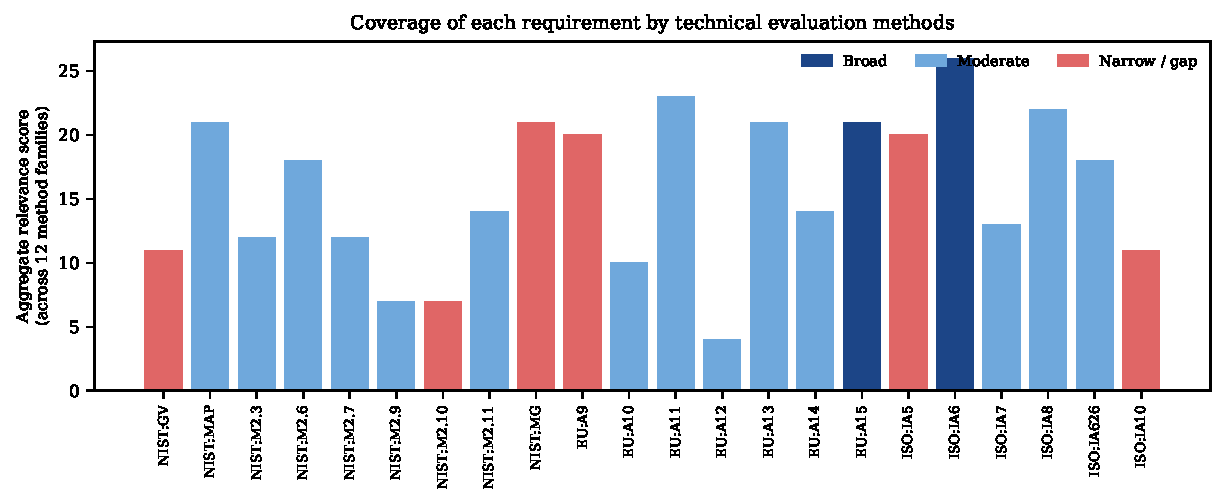
\includegraphics[width=0.92\textwidth]{../figures/fig_gap.pdf}
\caption{Aggregate coverage of each requirement by technical evaluation methods, colored
by coverage breadth. Bar height is the aggregate relevance score (primary${=}3$,
supporting${=}2$, contextual${=}1$, none${=}0$) summed across the twelve method families;
coverage breadth is set by the count of families with \emph{primary} relevance
(broad ${\geq}3$, moderate $1$--$2$, narrow $0$). \textbf{Takeaway:} a tall bar shaded
\emph{narrow} (e.g., NIST \textsc{Govern}, EU Article~9) has ample supporting evidence but
\emph{no} method of primary relevance---so the real gaps are process obligations,
human-oversight effectiveness, and agentic behavior, not the measurable
characteristics.}\label{fig:gap}\end{figure*}
Reading the mapping matrix by column rather than by row reveals where the technical
evaluation literature is rich and where it is thin relative to what the frameworks
demand. Table~\ref{tab:gap} summarizes the coverage breadth of evidence for each requirement, and
Fig.~\ref{fig:gap} visualizes the aggregate. We characterize coverage breadth by the
number of method families with \emph{primary} relevance: \emph{broadly covered} requirements
have several such families, \emph{moderately covered} ones one or two, and
\emph{narrowly covered} ones none.

\subsection{Well-served requirements}
The requirements most tightly coupled to the technical literature are those framed as
measurable trustworthiness characteristics: accuracy and performance, robustness,
security, explainability, and fairness. These correspond to NIST \textsc{Measure}~2.x,
EU AI Act Article~15, and the ISO/IEC~42001 verification-and-validation control. The
omnibus technical requirements that draw on several method families at once---EU
Article~15 (accuracy, robustness, and cybersecurity) and ISO/IEC~42001 A.6.2.4
(verification and validation)---reach the highest evidentiary coverage in our scheme
(``broad'' in Table~\ref{tab:gap}), while each individual trustworthiness characteristic
has primary relevance from one or more established method families. For systems built from
well-studied model classes on tabular or vision data, a deployer can today assemble
strong conformity evidence for these obligations using off-the-shelf methods.

\subsection{Process obligations: a definitional boundary, not a methods gap}
A first category is a structural boundary rather than a deficiency in the literature.
Obligations written as \emph{processes}---NIST \textsc{Govern}, EU AI Act Article~9 (the
risk-management system), and the ISO/IEC~42001 management-system clauses---are, by design,
not the kind of thing any single technical evaluation can satisfy. This is not an absence
of methods: documentation (M8, M9) and monitoring (M11) supply substantial evidence
\emph{inputs} to these processes, and the matrix records those supporting and primary
contributions. What process obligations require in addition is an organizational process
that integrates the technical evidence; the ``gap'' is therefore the need for such
integration, not missing measurement. We flag this so practitioners do not mistake a strong
benchmark report for conformity with a process obligation, and we reserve the term
\emph{gap} (below) for requirements that genuinely lack primary-relevance technical methods.

A second, more troubling gap concerns obligations for which a technical evaluation
\emph{should} exist but the methods are immature. \emph{Human-oversight effectiveness}
(EU Article~14) is the clearest case: although a human-in-the-loop is mandated, methods
for evaluating whether oversight is \emph{effective} (whether humans exhibit automation
bias, rely appropriately, or can actually intervene) are nascent~\cite{guo2024reliance,%
chen2024reliancedrills,romeo2025automationbias}. \emph{Record-keeping and logging} (EU
Article~12) is an engineering capability that, in practice, lacks evaluation methods for
assessing whether logs are adequate to reconstruct system behavior. \emph{AI impact
assessment} (ISO/IEC~42001 A.5; EU fundamental-rights impact assessment) has frameworks
but few standardized, quantitative evaluation instruments.

\subsection{The agentic measurement gap}
A significant and rapidly growing gap is created by the shift from models to agents.
Current evaluation methods overwhelmingly grade \emph{outputs}---the text a model emits in
response to a probe---whereas the risks of autonomous, tool-using systems arise from
\emph{actions}: which tools are invoked, which sub-agents are delegated to, how a plan
allocates resources. This is not a speculative concern: independent work shows that a
system near-parity on a question-answering fairness benchmark can still act with disparity
when it selects tools or escalates cases~\cite{li2025actions,blankenstein2025biasbusters},
that agent safety must be assessed over multi-step behavior rather than single
responses~\cite{zhang2024agent}, and that tool-integrated agents open attack surfaces (e.g.,
indirect prompt injection) absent in the base model~\cite{greshake2023notwhat}; dedicated
agent benchmarks are only beginning to appear~\cite{gu2025safesearch,peng2025eu}. Of our
corpus, only a small number of references evaluate action-level behavior, confirming the
class is under-covered. A recent framework (citation withheld for double-blind review) offers
one formalization of this measurement gap (token-level parity coexisting with action-level
disparity), but the gap stands on the independent evidence above. What is novel here is not
the individual agent benchmarks, which we cite, but the systematic identification of this
gap as a \emph{structural} mismatch between frameworks drafted for model-level evaluation
and the deployment reality of agentic, tool-integrated systems, surfaced by reading the
cross-framework matrix by column. Because the EU AI Act,
NIST AI RMF, and ISO/IEC~42001 were drafted with model-centric assessment in mind, their
requirements are presently evidenced by methods that do not observe the behaviors most
likely to cause high-risk harm in agentic deployments. Action-level evaluation harnesses,
trajectory logging tied to the logging obligations, and agentic red-teaming are, on the
evidence above, the most critical near-term directions for aligning technical evaluation
with regulatory intent (Section~\ref{sec:future}).

% Gap-analysis table (Table T5).
\begin{table}[t]
\centering
\caption{Gap analysis: \emph{coverage breadth} of technical evaluation evidence per requirement, with the principal gaps. Coverage breadth counts how many method families supply \emph{primary}-relevance evidence in Table~\ref{tab:matrix}: broad ($\geq$3 families), moderate (1--2), narrow (0). It measures breadth of mapped families, not the methodological maturity or validation quality of the underlying methods. \textbf{Takeaway:} the narrowly-covered requirements are consistently \emph{process} obligations (NIST \textsc{Govern}, EU Article~9, ISO A.5/A.10) and the obligations whose evaluation methods are immature (oversight effectiveness, logging adequacy), not the measurable trustworthiness characteristics.}
\label{tab:gap}
\footnotesize
\begin{tabular}{p{0.10\columnwidth}p{0.30\columnwidth}p{0.16\columnwidth}p{0.30\columnwidth}}
\toprule
FW & Requirement & Coverage breadth & Principal gap\\
\midrule
NIST & NIST GOVERN & Narrow & Governance is process-oriented; technical eval contributes documentation evidence only.\\
NIST & ME 2.10 Priv. & Narrow & Privacy-evaluation methods (membership inference, differential privacy) are established but function as vulnerability tests; full privacy assurance for LLMs/agents is under-served.\\
NIST & ME 2.11 Fair & Moderate & Model-level fairness evaluation is well developed; action-level/agentic disparity measurement is a structural gap.\\
EU & Art.9 & Narrow & EU Article 9 risk management is a process obligation: technical evaluations are inputs to, not a substitute for, the risk-management system.\\
EU & Art.12 & Moderate & Logging/record-keeping is an engineering capability; few evaluation methods assess log adequacy for reconstruction.\\
EU & Art.14 & Moderate & Human-oversight effectiveness evaluation (automation bias, appropriate reliance) is nascent relative to the obligation.\\
ISO & A.5 Impact & Narrow & AI impact-assessment is a process obligation; methods exist but lack standardized, quantitative evaluation instruments, so no family has primary relevance.\\
ISO & A.10 3rd-pty & Narrow & ISO A.10 third-party and customer relationships is served by supplier-assurance processes; few technical evaluation methods are primarily relevant to it.\\
\bottomrule
\end{tabular}
\end{table}



\section{Discussion: Putting the Mapping to Work}
\label{sec:discussion}

The value of the methods\,$\times$\,requirements matrix lies less in its rows and columns than in how a practitioner uses them to convert scattered evaluation activity into structured conformity evidence. This section translates the mapping into an actionable playbook, illustrates it on a worked example, situates it within a US-led assurance ecosystem, and explains why a single evidence base can serve all three frameworks.

\subsection{A Conformity-Evidence Playbook}
We propose a four-step routine for assembling an evidence dossier directly from the matrix. \textit{First}, scope the system: classify it against the obligation triggers of each framework, namely the high-risk categories of the EU AI Act \cite{euaiact2024}, the outcome categories of the NIST AI RMF \cite{nist2023airmf}, and the management-system controls of ISO/IEC 42001 \cite{iso42001}, to determine which columns of Table~\ref{tab:matrix} are in scope. \textit{Second}, read down each in-scope column to enumerate the technical evaluation methods that can supply evidence for that requirement; the matrix thus acts as a requirements-to-tests index rather than a literature taxonomy. \textit{Third}, execute the selected methods and capture their outputs as durable artifacts (model cards \cite{puhlfurss2025modelcards}, system cards \cite{reddy2025systemcards}, audit cards \cite{staufer2025auditcards}, and technical documentation templates \cite{lucaj2025techops}), so that each evaluation produces a citable record rather than a transient result. \textit{Fourth}, reconcile coverage using the checklist in Table~\ref{tab:checklist}, which flags requirements with no associated evaluation evidence and exposes residual gaps before an assessor does. The dossier that emerges is a traceable chain from obligation to method to artifact, which is precisely the structure that certification proposals \cite{pan2024modelreporting} and automated compliance frameworks \cite{compliance2025pasta} assume but rarely make explicit.

\subsection{Worked Mini-Example}
Consider a hiring-screening model, which the EU AI Act treats as high-risk, triggering data-governance and accuracy-and-robustness duties \cite{euaiact2024}. Following the playbook, the in-scope columns include EU Art.~10 (data and data governance) and Art.~15 (accuracy, robustness, and cybersecurity). Reading down these columns, the practitioner selects dataset documentation and representativeness analysis to evidence Art.~10, and disaggregated accuracy testing, subgroup fairness evaluation, and adversarial robustness testing to evidence Art.~15; the fairness evaluations also speak to the non-discrimination questions that recent work shows are only partially captured by the Act's accuracy provisions \cite{meding2025algorithmicdiscrimination}. The same evaluations populate the NIST \textsc{Measure} function, whose analysis, benchmarking, and monitoring outcomes are evidenced by the identical test artifacts \cite{nist2023airmf}, and they supply evidence toward ISO/IEC 42001 controls A.6 (AI system life-cycle) and A.7 (data for AI systems) by producing records of documented, repeatable processes \cite{iso42001}. A clinical-decision model follows the same path with domain-specific robustness and monitoring evidence, illustrating how the matrix is intended to apply across high-risk application domains rather than encoding one sector's assumptions; we offer these as worked illustrations, not as a validation study.

\subsection{From a Test List to an Assurance Case}
A list of relevant tests is not yet an assurance case. To show how the crosswalk feeds one, we sketch a single assurance argument for the hiring model's Article~15 accuracy obligation, with the elements an assessor expects. \textit{Obligation:} EU AI Act Article~15 (appropriate accuracy). \textit{Scoped claim:} ``the system's selection accuracy and error rates are adequate and stable for the stated intended purpose and population.'' \textit{System context:} defined intended purpose, candidate population, and operating constraints. \textit{Evaluation protocol:} disaggregated accuracy and error-rate testing on a held-out, representative sample, with distribution-shift checks. \textit{Metric and acceptance criterion:} false-negative-rate parity within a pre-registered tolerance across protected groups, and overall accuracy above a domain-justified threshold; the criterion, not merely the test, is what discharges the claim. \textit{Result and uncertainty:} measured rates with confidence intervals. \textit{Residual risk:} performance on under-represented subgroups and post-deployment drift. \textit{Owner and cadence:} a named accountable role, with re-evaluation on each model or data change. The crosswalk locates \emph{which} evaluations are relevant; the assurance case adds the claim, context, threshold, uncertainty, residual risk, and sign-off that convert a relevant test into admissible evidence. This is the template practitioners should instantiate per obligation, and the layer a purely method-centric reading of the matrix omits.

\subsection{Evidence Levels and Stakeholders}
Two cautions keep the playbook from collapsing into checklist compliance. First, the \emph{unit of evaluation} matters: the same family yields evidence at the model level (e.g., a benchmark score), the system level (the model within its guardrails and tools), the workflow level (the human--AI process), and the organization level (governance and monitoring). High-risk conformity depends on the higher levels, yet most cited methods operate at the model level; practitioners should record, for each artifact, which level it actually evidences, and treat a model-level result as insufficient for a system- or workflow-level obligation. Second, conformity evidence implicates a \emph{stakeholder set} wider than the provider: deployers and operators (who run human oversight), affected persons (whose recourse and complaints can serve as evidence of oversight and fairness in practice), auditors and notified bodies (who judge sufficiency), regulators, and downstream integrators and third-party model vendors (whose dependencies must be represented). Human-oversight evidence in particular should distinguish the mere availability of a human from measured \emph{effectiveness} (detection, appropriate reliance, intervention success, escalation latency, authority, workload, training, and contestability), and should, where the obligation concerns affected persons, include evidence from operators and affected parties rather than from the model alone.

\subsection{US National-Importance Framing}
For a US audience, the playbook is most naturally anchored on the NIST AI RMF as the organizing spine, with the \textsc{Measure} function and the Generative AI Profile \cite{nist2024genai} supplying the evaluation vocabulary into which EU and ISO obligations are then translated. This NIST-centric framing matters for national competitiveness: a voluntary, outcome-based core lets US developers build one evaluation pipeline that also supports conformity evidence for export to regulated markets, an asymmetry that cross-regional studies highlight between voluntary and prescriptive regimes \cite{almaamari2025crossregional}. The framing also creates the demand-side conditions for an independent assurance market, in which third-party auditors verify evaluation claims rather than merely accept self-attestation \cite{auditing2024frontier}, and in which continuous-assurance postures extend point-in-time conformity to systems that evolve after deployment \cite{lupo2026trustworthyposture}.

\subsection{One Evidence Base, Three Frameworks}
The deeper implication of Table~\ref{tab:matrix} is that the three frameworks are largely non-redundant \textit{in obligation} yet highly overlapping \textit{in evidence}: in our mapping, all twelve method families have primary or supporting relevance to requirements in all three frameworks (Table~\ref{tab:matrix}), so no family is specific to a single regime. Because a single robustness test or fairness audit can be cited against a NIST outcome, an EU article, and an ISO control simultaneously, the marginal cost of multi-framework conformity is far lower than the number of frameworks would suggest, an economy that crosswalk efforts between the AI Act and international standards have begun to formalize \cite{hernandez2024knowledgegraph}, and that ISO/IEC 23894 risk guidance reinforces \cite{iso23894}. The practitioner's task therefore shifts from running parallel compliance programs to maintaining one well-documented evaluation base and re-indexing its artifacts against each framework's vocabulary, which is the central operational claim this review advances.

% T7 — practitioner conformity-evidence checklist
\begin{table*}[!tp]
\centering
\caption{Practitioner conformity-evidence checklist. For each cross-framework obligation
cluster, the recommended technical evaluation evidence and the supplying method family.
Clause identifiers are indicative; deployers must confirm applicability to their system. \textbf{Takeaway:} each obligation cluster maps to a small, named set of evaluations and a single supplying family, so one well-documented evidence dossier can be re-indexed against all three frameworks at once.}
\label{tab:checklist}
\footnotesize
\begin{tabular}{p{0.22\textwidth}p{0.40\textwidth}p{0.13\textwidth}p{0.16\textwidth}}
\toprule
Obligation cluster & Recommended technical evidence & Family & Clauses (NIST / EU / ISO)\\
\midrule
Accuracy \& performance & Held-out and OOD test results with metrics, confidence intervals, calibration & M1, M7 & ME 2.3 / Art.15 / A.6.2.4\\
Robustness \& security & Adversarial-robustness tests, red-team/jailbreak reports, certified bounds where feasible & M3, M5 & ME 2.6--2.7 / Art.15 / A.6.2.4\\
Fairness \& non-discrimination & Subgroup performance, bias-benchmark results, counterfactual/action-level disparity & M2 & ME 2.11 / Art.10,15 / A.5\\
Data governance & Datasheets/data cards, provenance and contamination audits, representativeness analysis & M8 & MAP / Art.10 / A.7\\
Transparency \& documentation & Model/system card, technical documentation dossier (Annex IV), FactSheet & M9 & ME 2.8 / Art.11,13 / A.8\\
Explainability & Attribution/explanation outputs with faithfulness evaluation & M6 & ME 2.9 / Art.13 / A.6.2.4\\
Human oversight & Oversight-effectiveness and appropriate-reliance evidence, escalation paths & M10 & GOVERN / Art.14 / A.9\\
Risk management (process) & The above, organized into a documented risk-management/impact-assessment process & all & GOVERN/MANAGE / Art.9 / A.5\\
Privacy & Membership-inference/extraction testing, differential-privacy guarantees, model-inversion resistance & M12 & ME 2.10 / Art.10 / A.7\\
Post-market monitoring & Drift/runtime monitors, logging, incident reporting, continuous re-evaluation & M11 & MANAGE / Art.12,72 / A.6.2.6\\
\bottomrule
\end{tabular}
\end{table*}


\section{Limitations and Threats to Validity}\label{sec:limits}
We record the threats to the validity of this review and the limitations of the mapping.

\textbf{Interpretive construct validity.} The frameworks are written at the level of
outcomes and processes and do not prescribe methods. Our (method, requirement) evidence
strengths are therefore reasoned engineering interpretations, not legal compliance
determinations. We mitigated subjectivity with an adversarial second pass over every
non-blank cell and by grounding each assignment in the official clause text, but
reasonable experts may code individual cells differently. The matrix should be read as a
structured argument, not an authoritative legal crosswalk.

\textbf{Temporal validity.} All three frameworks are moving targets. EU AI Act delegated
acts and the CEN--CENELEC harmonised standards are still in progress; US executive-branch
AI policy has shifted over the review window; and ISO/IEC companion standards continue to
emerge. The mapping is a snapshot dated June~2026 and is intended to be maintained as a
living artifact (Section~\ref{sec:future}).

\textbf{Selection and search bias.} Despite a broad, multi-source search, database
coverage, English-only inclusion, and the inclusion of preprints introduce bias. The
reused agent-fairness corpus is, by construction, dense in fairness methods (M2); other
families draw on a newer, smaller verified set, which may under-represent some mature
methods. We report counts transparently rather than claiming exhaustiveness.

\textbf{Citation integrity.} Cited references were verified against arXiv abstract-page
resolution, the Consensus database, or official DOIs where resolvable, and the corpus was
de-duplicated; the verification caught and corrected a substantial fraction of initially
mis-attributed metadata. We do not claim exhaustive verification of every entry in the
released corpus, and residual risk remains for the newest preprints whose venues may change.

\textbf{Not legal advice.} This article is a technical review for evaluation
practitioners and researchers. It does not constitute legal advice, and conformity
determinations remain the responsibility of providers, deployers, notified bodies, and
competent authorities.


\section{Open Challenges and Future Directions}\label{sec:future}
The gap analysis points to a concrete research and standardization agenda. We organize it
by priority.

\textbf{Action-level evaluation for agentic systems.} The agentic measurement gap
(Section~\ref{sec:gaps}) is the most urgent. The field needs evaluation harnesses that
instrument an agent's \emph{trajectory}---tool calls, delegations, plan steps---and
compute disparity, safety, and reliability over actions rather than tokens. Such
harnesses would simultaneously serve EU Article~12 logging, Article~14 oversight, and
NIST \textsc{Manage} monitoring, turning a compliance burden into a measurement
substrate.

\textbf{Standardized conformity evaluations and harmonised benchmarks.} At present,
mapping a method to a requirement still requires expert interpretation. The natural next
step is \emph{harmonised standards}---the CEN--CENELEC deliverables anticipated by the EU
AI Act, and NIST/ISO test methods---that fix, for each obligation, a reference evaluation
protocol and an acceptance criterion. A living, versioned benchmark registry tied to
specific clauses would reduce the interpretive latitude that our matrix currently
documents.

\textbf{Evaluation of process and oversight obligations.} The under-served, non-process
gaps---oversight effectiveness, log adequacy, impact-assessment quality---call for new
evaluation \emph{methods}, not merely new documentation. Human-subjects protocols for
appropriate reliance, log-reconstruction audits, and quantitative impact-assessment
instruments would convert today's documentary evidence into measurable evidence.

\textbf{Third-party audit and assurance ecosystems.} Conformity assessment ultimately
depends on credible, independent evaluation. Recent work on rigorous third-party auditing
of frontier developers~\cite{auditing2024frontier} and scalable multi-policy compliance
evaluation~\cite{compliance2025pasta} points toward an assurance ecosystem; in the US,
this aligns with a NIST-anchored, voluntary-conformity model of national importance for
AI safety and governance.

\textbf{Automated and continuous evidence generation.} As models and regulations both
evolve, one-shot evaluation is insufficient. Continuous-assurance pipelines that
re-generate conformity evidence on each model or data update---and that flag when a prior
evaluation has been invalidated by drift---would keep the evidence base current and
directly serve post-market monitoring obligations.

\textbf{A living mapping.} Finally, because the frameworks themselves evolve, the mapping
in this article is a snapshot. We intend to maintain it as a versioned, machine-readable
companion artifact so that the community can extend, correct, and re-time the
method-to-requirement assignments as standards mature and new evaluation methods appear.


\section{Conclusion}\label{sec:conclusion}
High-risk AI systems must now demonstrate conformity with overlapping governance
frameworks, yet the technical evaluation literature and the regulatory requirements have
developed in separate worlds. This article bridged them. We organized the AI-evaluation
literature into twelve method families and mapped each, graded by technical relevance, to
the requirements of the NIST AI RMF, the EU AI Act high-risk obligations, and ISO/IEC
42001---producing, to our knowledge, the first crosswalk of evaluation methods to the
simultaneous requirements of the three frameworks within the technical literature we surveyed. The
resulting matrix shows that measurable trustworthiness characteristics (accuracy,
robustness, security, explainability, fairness) are broadly covered by established methods, that the
same evaluation artifact is often relevant to all three frameworks at once, and that process
obligations, human-oversight effectiveness, logging adequacy, and---most critically---the
behavior of agentic systems remain weakly served by current technical methods. We offered a
practitioner playbook for assembling a cross-framework evidence dossier and a research
agenda led by action-level evaluation for agents. Cited references and regulatory claims
were verified against official and primary sources where publicly accessible, and the
coding artifacts are released for external scrutiny. The mapping is a structured,
auditable argument graded by technical relevance---not a deterministic compliance tool; final
conformity determinations remain the responsibility of providers, deployers, and notified
bodies, and the mapping does not constitute legal advice. We release the
mapping as a living, machine-readable artifact in the hope that it becomes a durable
reference as both AI evaluation methods and AI regulation continue to mature.


\input{acknowledgment.tex}

\clearpage  % flush any pending floats so no tables/figures trail after the references

\bibliographystyle{IEEEtran}
\bibliography{../references}

\input{biographies.tex}

\end{document}
